\documentclass[ngerman]{beamer}
\usetheme{metropolis}

% use \cref instead of autoref, autoref does not work with beamer
\usepackage{cleveref}

\usepackage{appendixnumberbeamer}


% some imports from handout, probably dont need all but whatever
\usepackage[utf8]{inputenc}
\usepackage[T1]{fontenc}   
\usepackage{graphicx}       
\usepackage[german]{babel}
\usepackage{csquotes}     
\usepackage{eurosym}
\usepackage{float}
\usepackage{rotating}
\usepackage{blkarray}
\usepackage{amsmath}
\usepackage{amssymb}
\usepackage{gensymb}
\usepackage{amsthm}
\usepackage{listings}
\usepackage{caption}
\usepackage{subcaption}
\usepackage{interval}
\usepackage{textpos}
\usepackage{xcolor}
\usepackage{tabularx}
\usepackage[style=authoryear, backend=biber]{biblatex}
\usepackage{graphics}
\addbibresource{references.bib}


% argmin command
\newcommand{\argmin}[1]{\underset{#1}{\operatorname{arg}\,\operatorname{min}}\;}
% command for euclidean norm
\newcommand{\norm}[1]{\lVert#1\rVert}
% command for lagrangian L (kind of handwritten L)
\newcommand{\Lagr}{\mathcal{L}}

% show current page number in footer
\setbeamertemplate{footline}[frame number]


% No navigation symbols at the slides' bottom
\beamertemplatenavigationsymbolsempty

% command for creating a frame with one full-slide image without caption
% first arg: frame title, second arg: path to img
\newcommand {\imageframe}[2] {
	\begin{frame}{#1}
		\begin{center}
			\begin{figure}
			\includegraphics[width=\textwidth,height=0.8\textheight,keepaspectratio]{#2}
		\end{figure}
		\end{center}
	\end{frame}
}



\title{Support Vector Machines}
\author{André Hopfgartner \& Matthias Rupp}
\institute{Vorarlberg University of Applied Sciences \\ \\ \\ \\ \\ \\ 
\includegraphics[width=0.35\textwidth]{assets/Logo-A3.png}}

\date{08.06.2021}

\begin{document}

\begin{frame}[plain]
    \maketitle
\end{frame}


\begin{frame}{Agenda}
	\setbeamertemplate{section in toc}[sections numbered]
	\tableofcontents[hideallsubsections]
\end{frame}


\section{Einführung}


\begin{frame}{Intuition}
	\emph{Ziel}: lineare Trennung zweier Klassen\\ \pause
	\emph{Wie?}: Definition einer (Hyper-) Ebene \\ \pause
	\emph{Nebenbedingung}: Möglichst großer freier Bereich\\ \pause
	
	\begin{center}
		\begin{figure}
			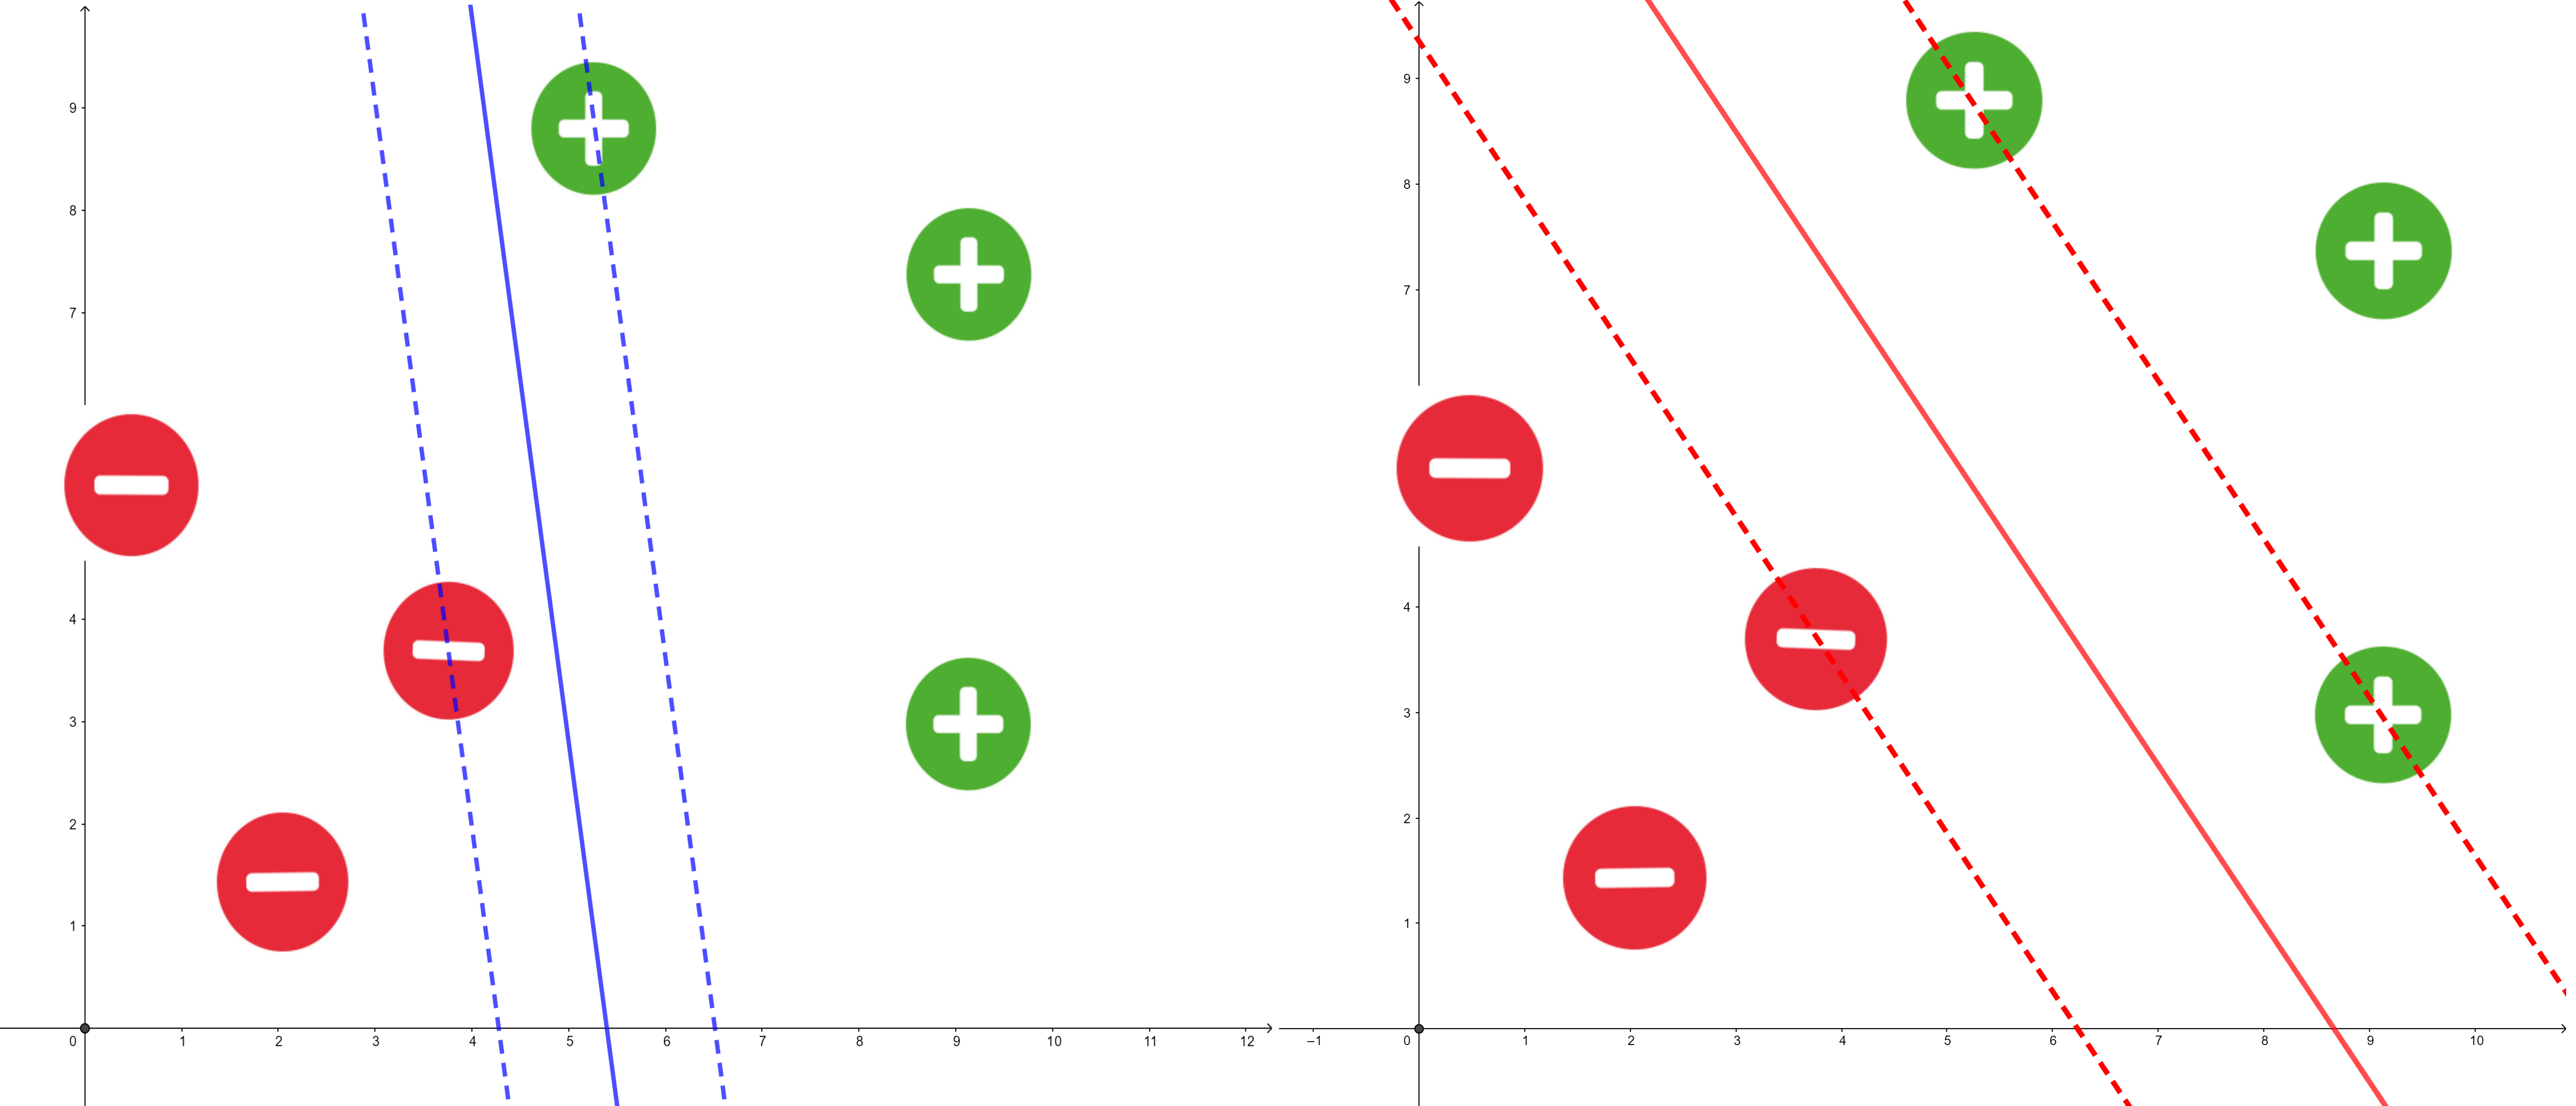
\includegraphics[width=\textwidth,height=0.7\textheight,keepaspectratio]{assets/small_vs_big_margin.png}
		\end{figure}
	\end{center}	
\end{frame}

\begin{frame}{Arten von SVM}
	\emph{Arten von SVM:}
	\begin{itemize}
		\item \emph{Hard-Margin SVM}: Daten werden 100\% korrekt getrennt
		\item \emph{Soft-Margin SVM}: Einzelne Datenpunkte können falsch klassifiziert werden um insgesamt bessere Trennung zu erhalten
	\end{itemize}

	\begin{center}
		\begin{figure}
			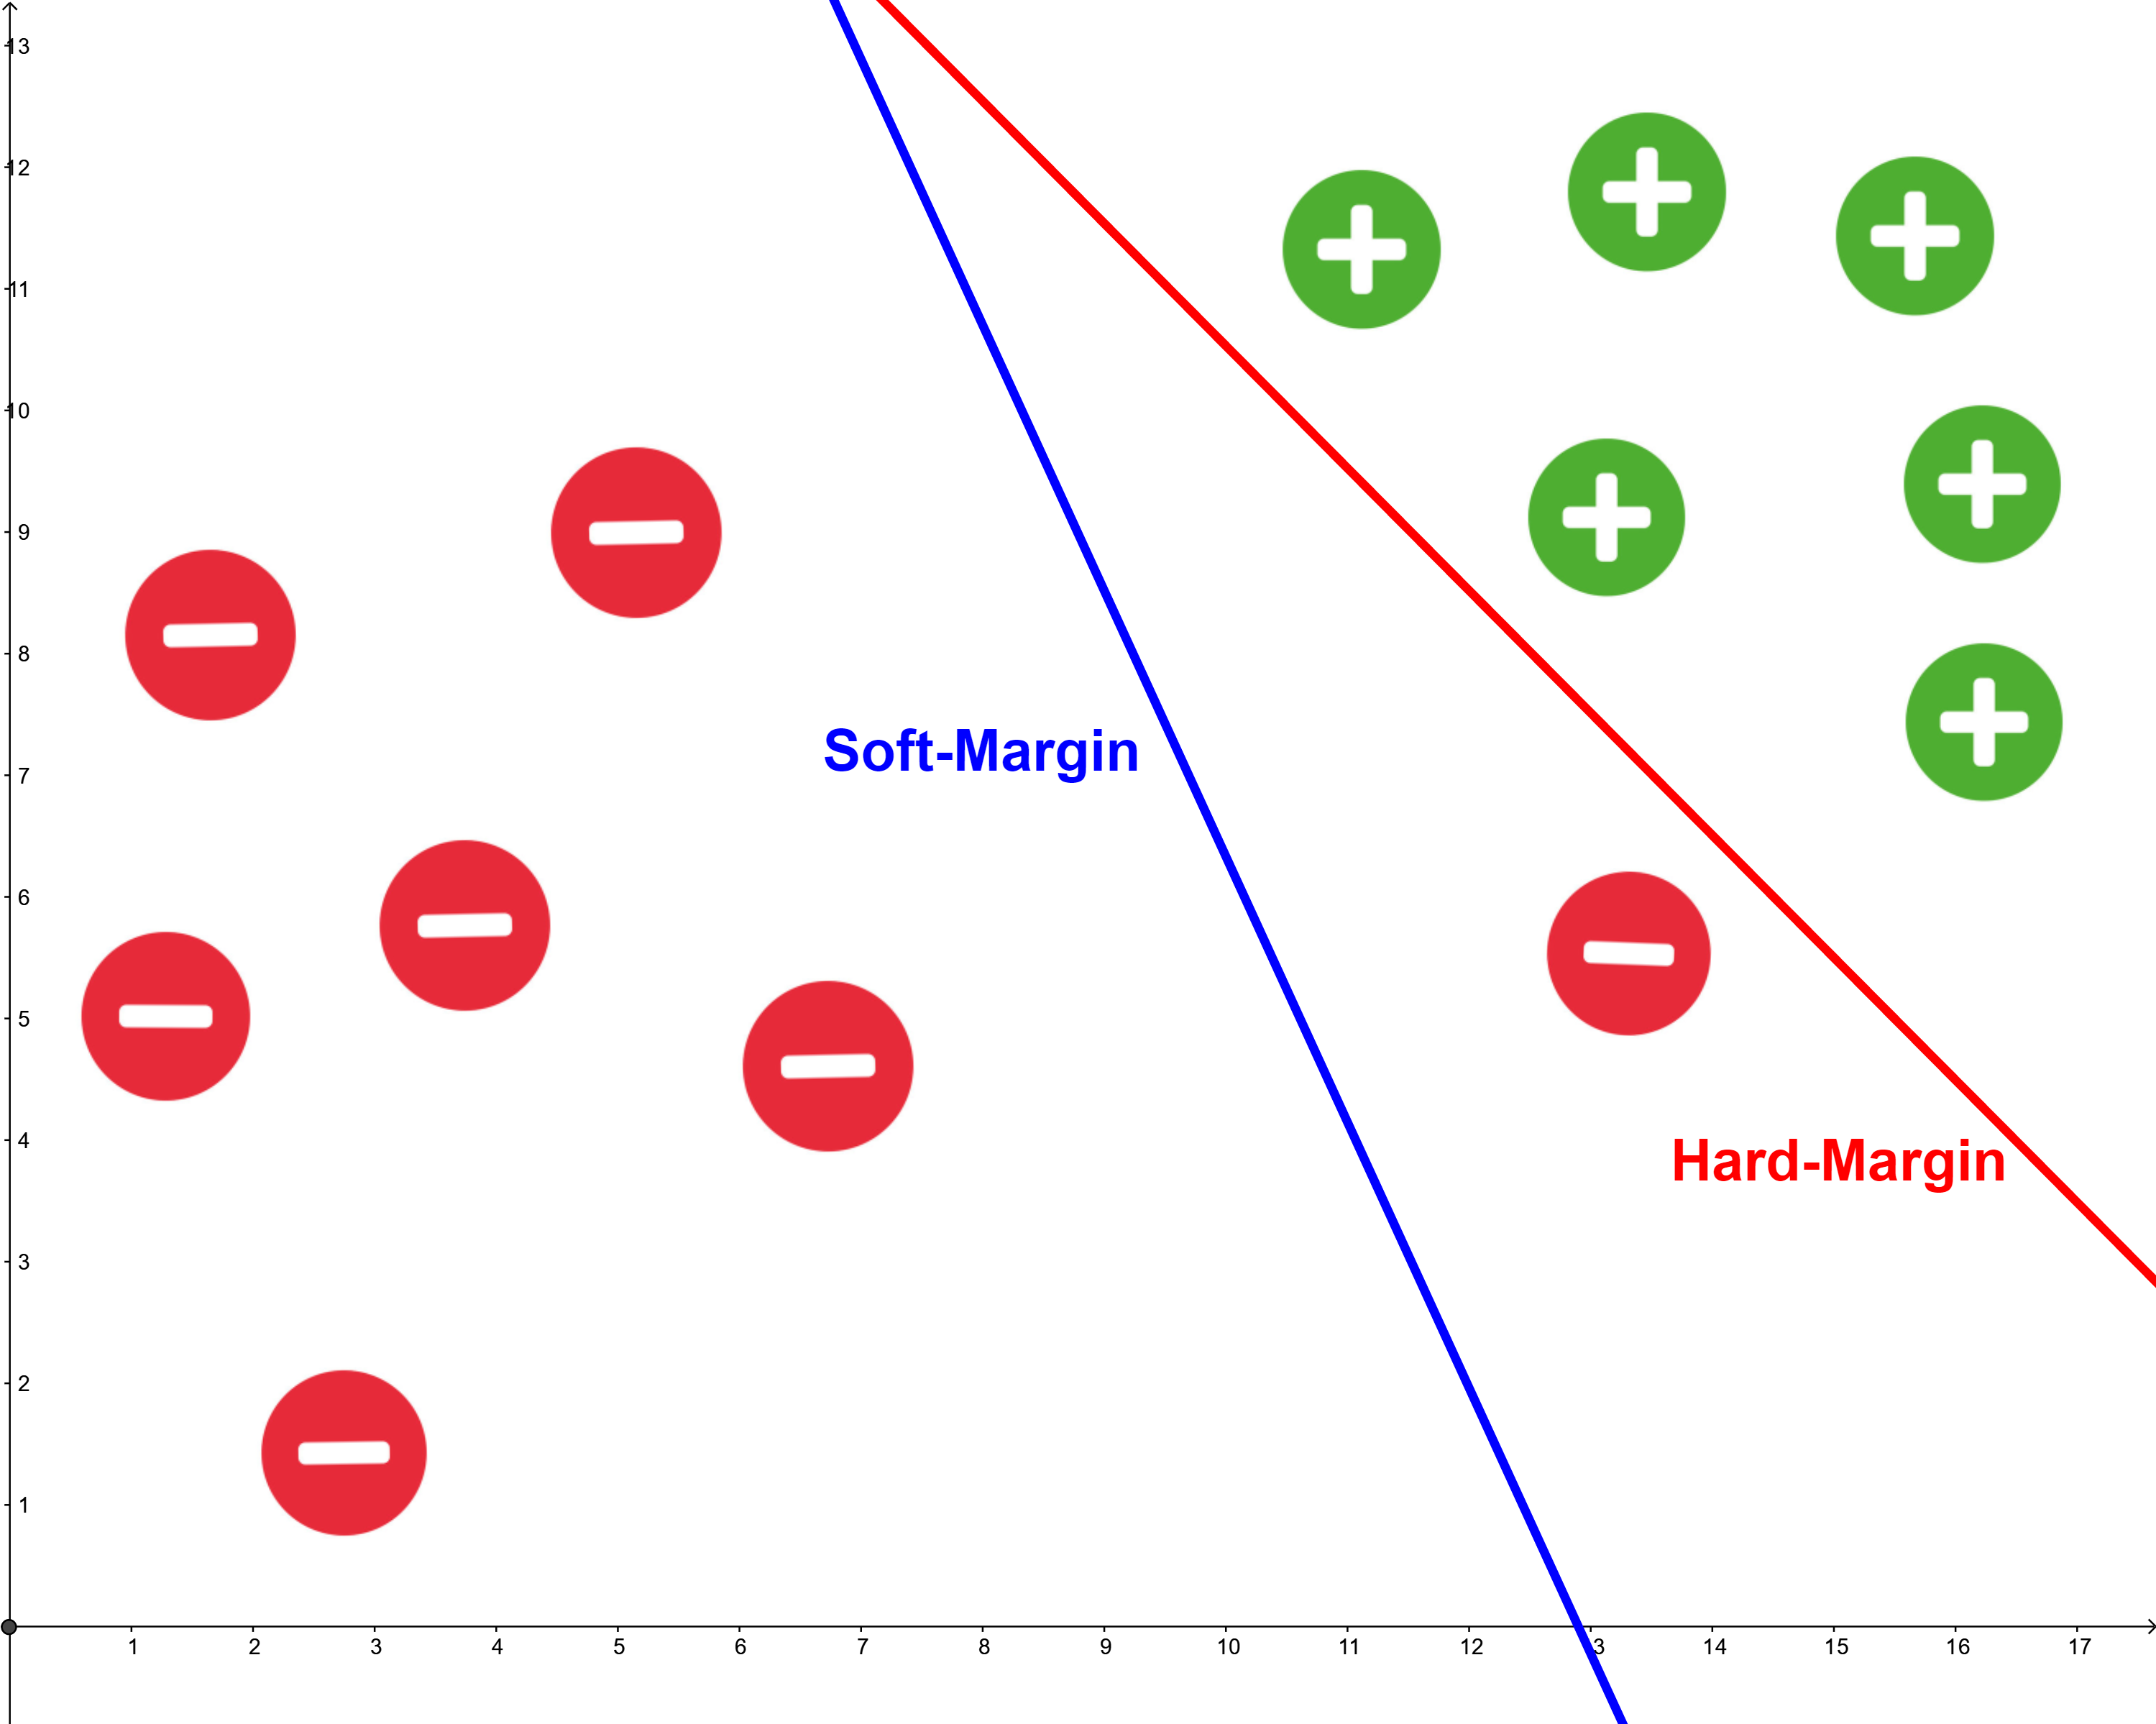
\includegraphics[width=\textwidth,height=0.6\textheight,keepaspectratio]{assets/hard_vs_soft_margin.png}
		\end{figure}
	\end{center}

\end{frame}

\section{Hard-Margin Support Vector Machine}


\begin{frame}{Mathematische Formulierung}
Gegeben sei ein Gewichtsvektor $w \in \mathbb{R}^{K}$, ein Bias $b \in \mathbb{R}$, ein beliebiger Punkt $x_{n} \in \mathbb{R}^{K}$ und ein zugehöriges Label $y_{n} \in \{-1, +1\}$. Eine Ebene im Raum kann allgemein definiert werden durch:

\begin{equation*} \label{plane_eq}
	\begin{aligned}
		w^{T} x_{n} + b &= 0 \\
	\end{aligned}
\end{equation*}

Ziel der SVM: $w$ und $b$ bestimmen für optimale Trennung

\end{frame}


\begin{frame}{Klassifikation}
	Annahme: $w$ und $b$ bereits bekannt\\
	Wie klassifiziert man einen Punkt $x_{n}$? \\ \pause
	Liegt $x_{n}$ über oder unter Ebene = Vorzeichen:
	\begin{subequations}
		\begin{alignat*}{2}
			y = sign(w^{T} x_{n} + b)  & \qquad & \text{ ist gleichbedeutend mit} \\
			w^{T} x_{n} + b > 0 & & \text{ für } y_{n} = +1\\
			w^{T} x_{n} + b < 0 & & \text{ für } y_{n} = -1
		\end{alignat*}
	\end{subequations}

	Bisher: Punkte können genau auf der Grenze liegen wenn $w^{T} x_{n} + b = 0$ \\
\end{frame}



\begin{frame}{Einführung eines Trennbandes}	
	Striktere Regel: Um Ebene soll Band frei bleiben \\
	\begin{subequations} \label{decision_rules}
		\begin{alignat*}{2}
			w^{T} x_{n} + b \geq +1 & \qquad & \text{ für } y_{n} = +1\\
			w^{T} x_{n} + b \leq -1 & & \text{ für } y_{n} = -1
		\end{alignat*}
	\end{subequations}

	\begin{center}
		\begin{figure}
			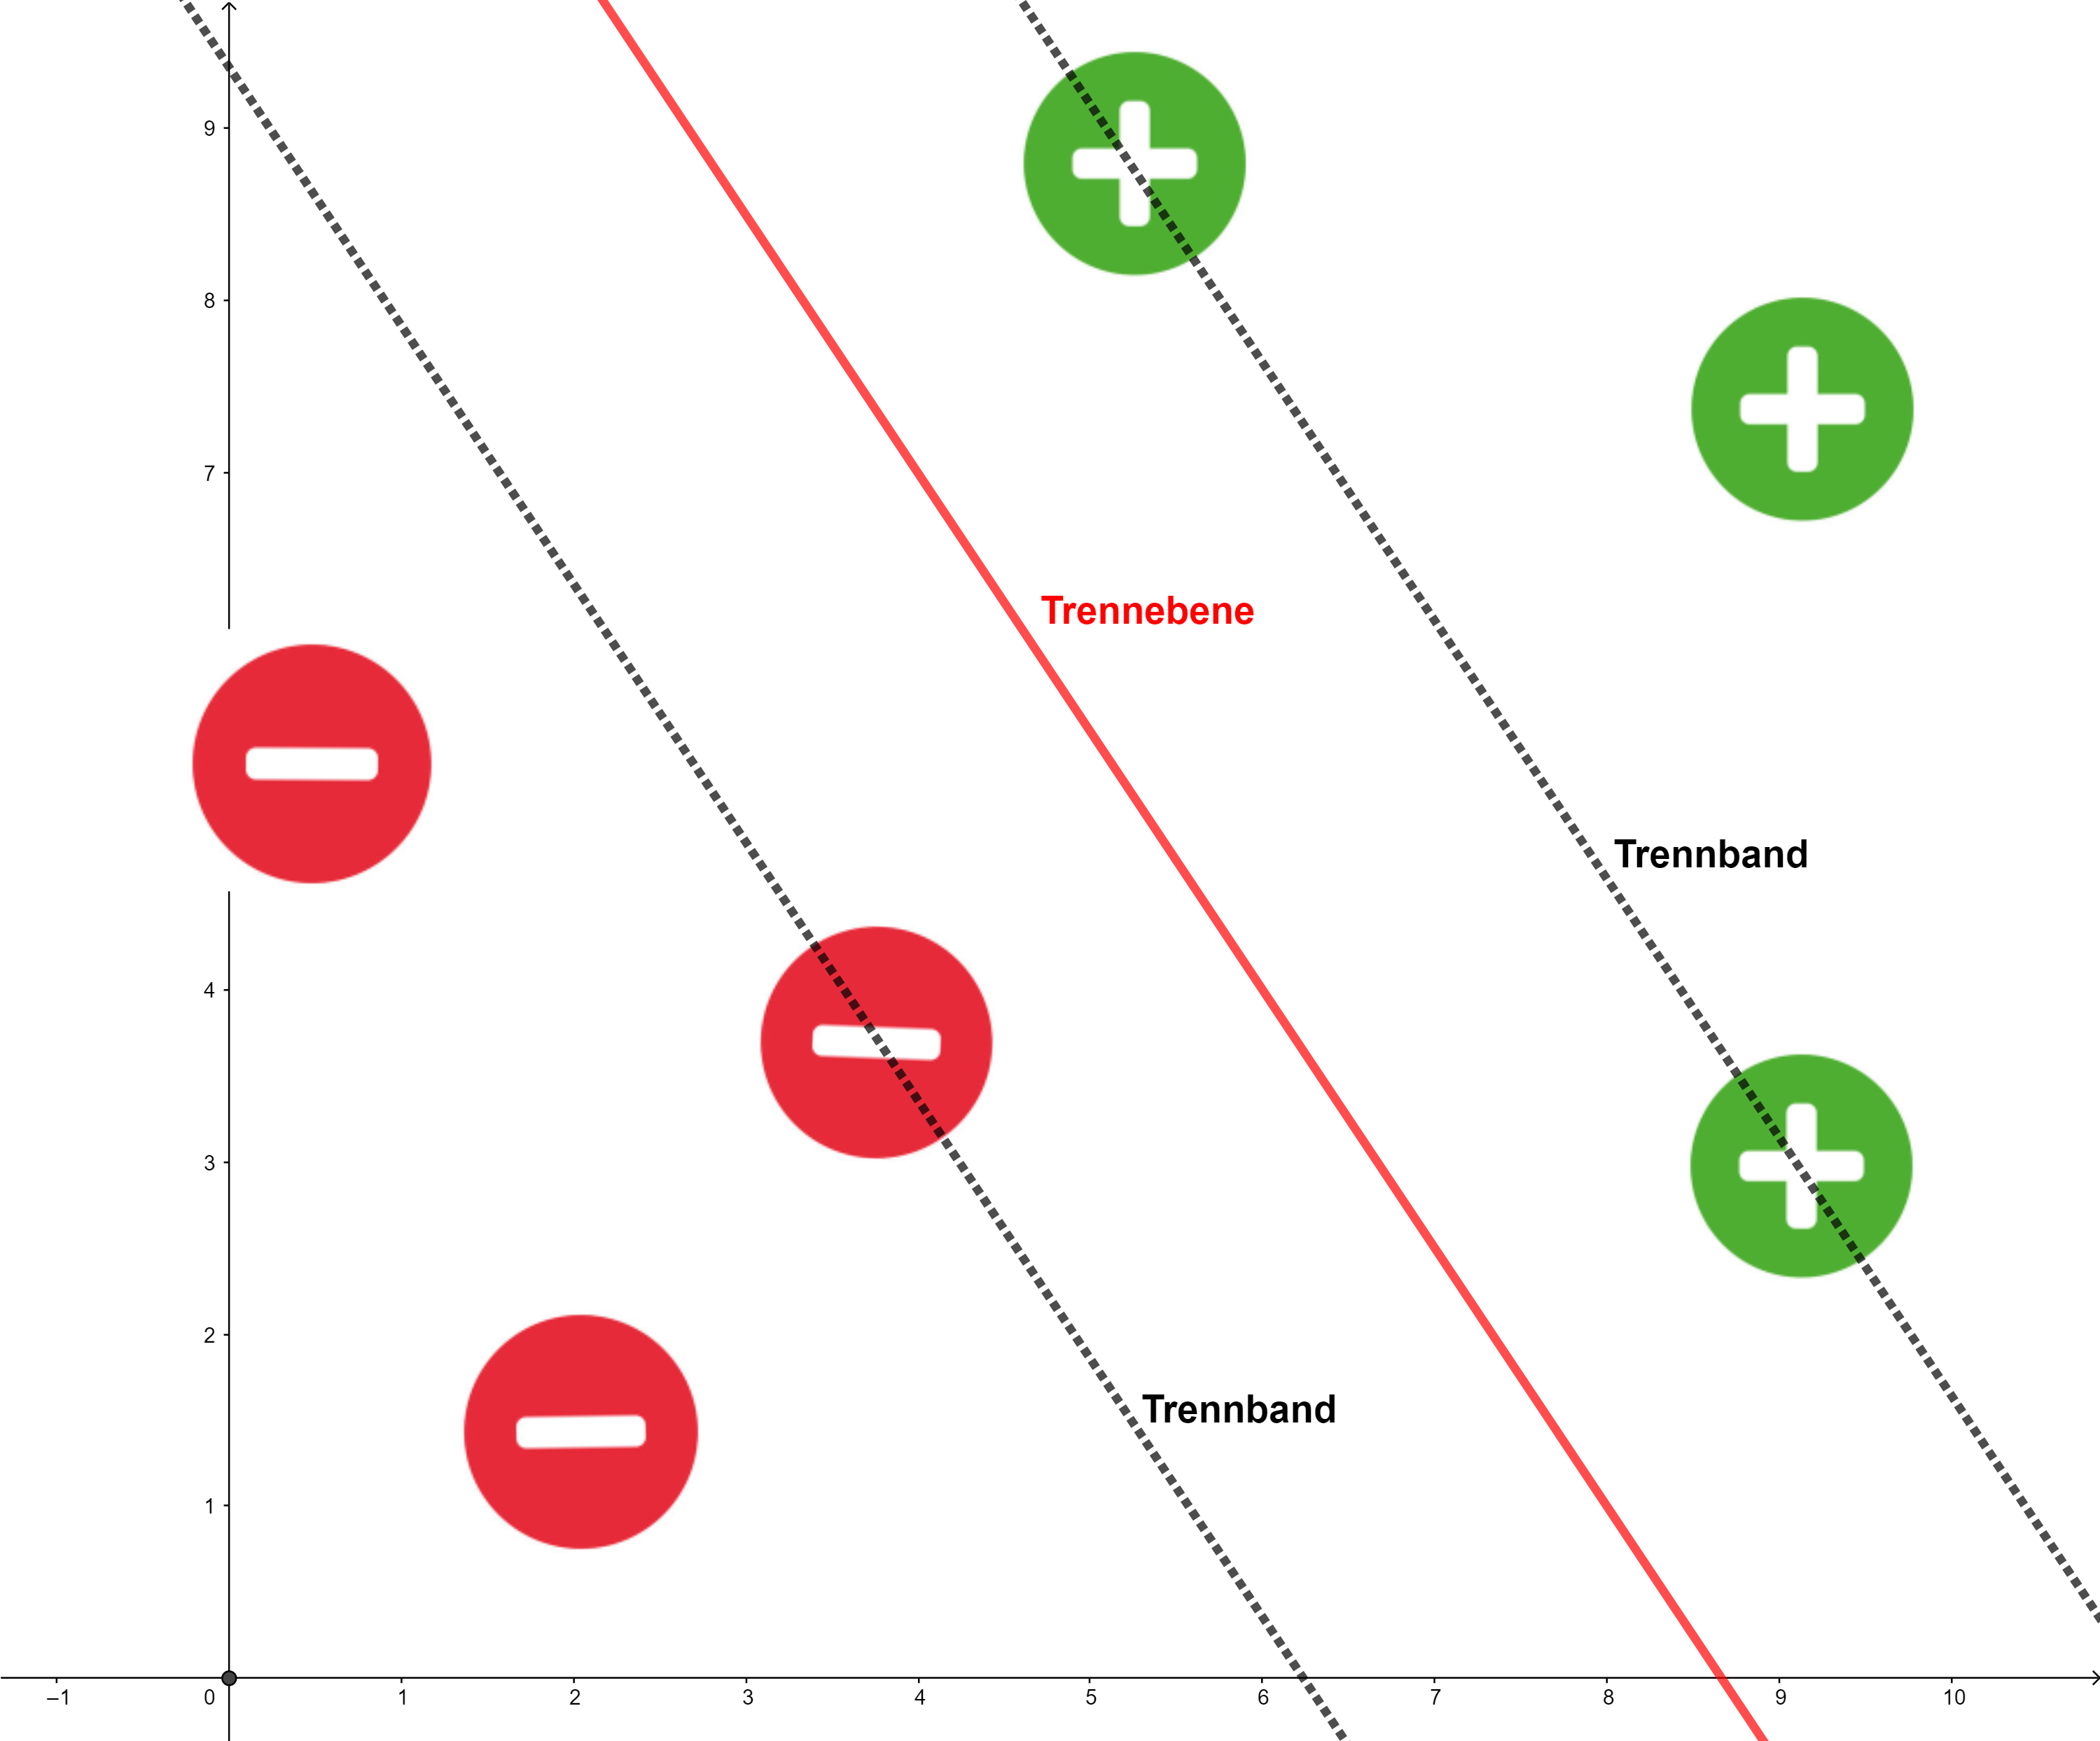
\includegraphics[width=\textwidth,height=0.6\textheight,keepaspectratio]{assets/trennband.png}
		\end{figure}
	\end{center}

\end{frame}

\begin{frame}{Einführung eines Trennbandes}
	Beidseitige Multiplikation mit $y_{n}$
	\begin{subequations}
		\begin{alignat*}{2}
			y_{n} (w^{T} x_{n} + b) \geq 1 & \qquad & \text{ für } y_{n} = +1\\
			y_{n} (w^{T} x_{n} + b) \geq 1 & & \text{ für } y_{n} = -1
		\end{alignat*}
	\end{subequations}

	\pause 
	Für den Fall, dass $x_{n} = \hat{x}$ genau an der Grenze des Trennbands liegt, gilt somit:
	\begin{equation*}
		\begin{aligned}
			y_{n} (w^{T} \hat{x} + b) &= 1
		\end{aligned}
	\end{equation*}
\end{frame}



\begin{frame}{Normalabstand eines Punktes zur Ebene}
	Gesucht: Normalabstand $d$ eines Punktes $x_{n} \in \mathbb{R}^{K}$ zur Ebene \\
	
	\begin{center}
		\begin{figure}
			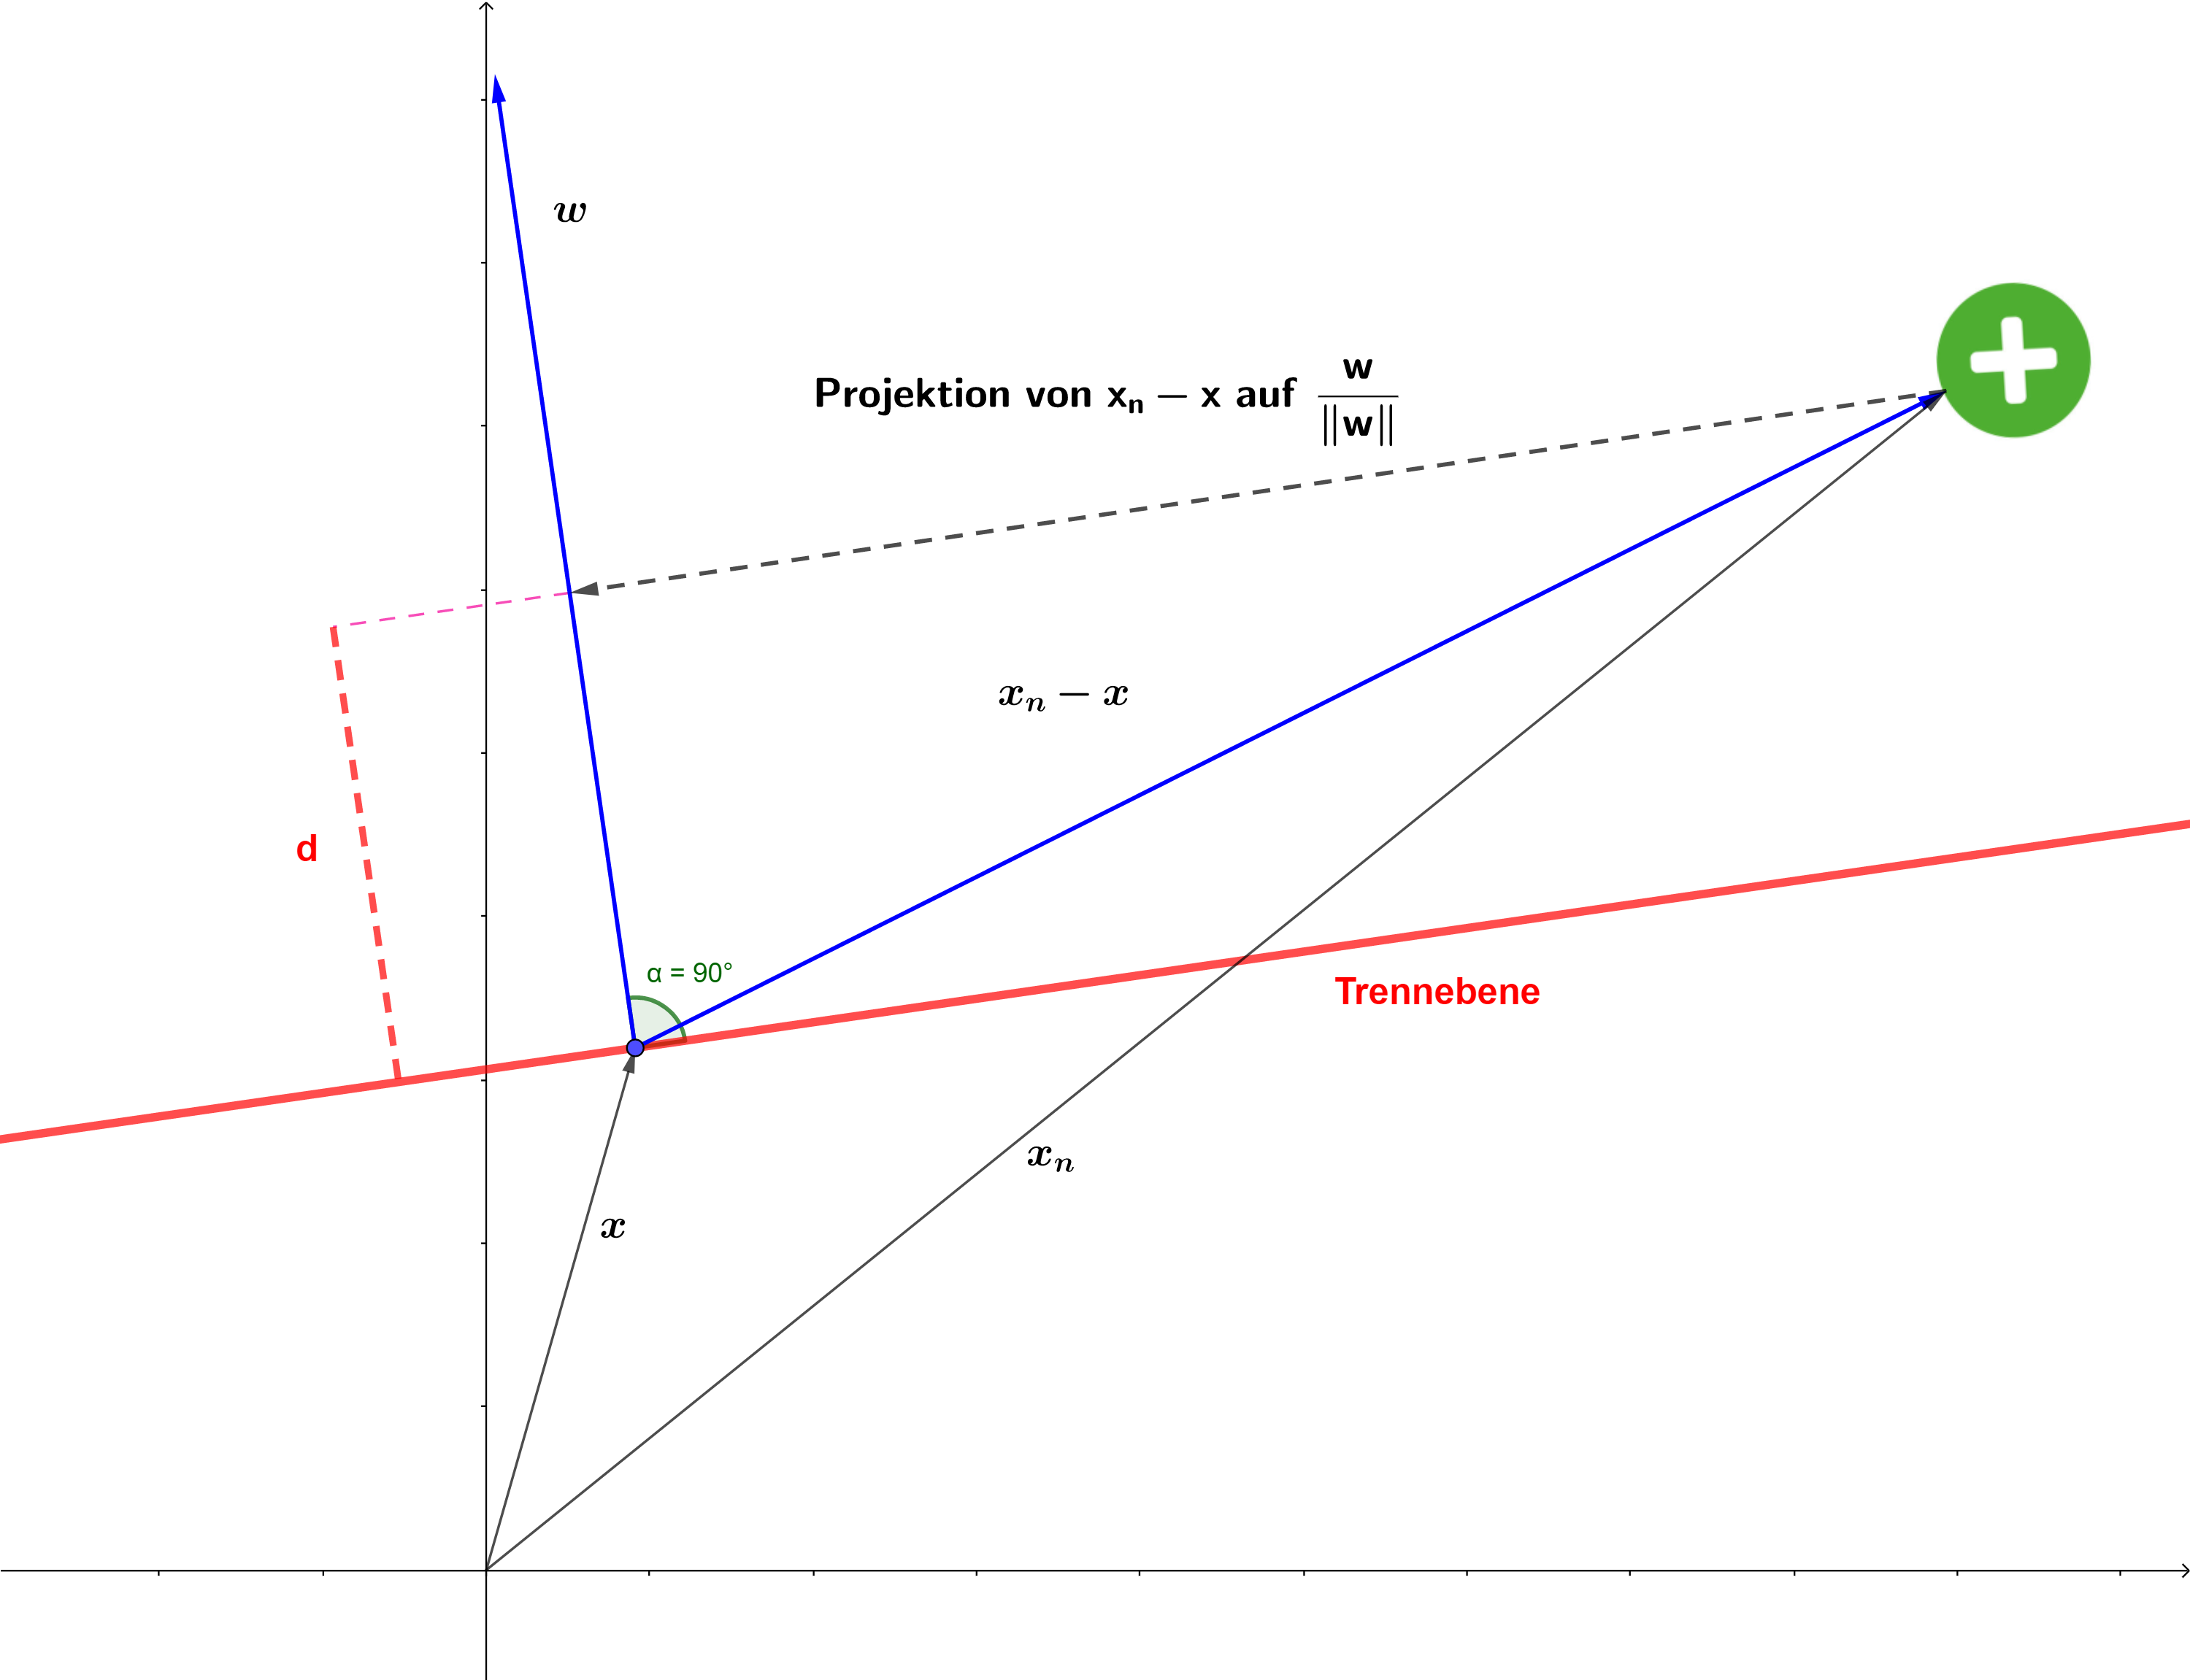
\includegraphics[width=\textwidth,height=0.8\textheight,keepaspectratio]{assets/projection.png}
		\end{figure}
	\end{center}
\end{frame}

\begin{frame}{Normalabstand eines Punktes zur Ebene}
	\begin{equation*}
		\begin{aligned}
			d &= | \frac{w^{T}}{\lVert w \rVert} (x_{n} - x) | = \\
			&= \frac{1}{\norm{w}} | (w^{T} x_{n} - w^{T} x) | =\\
			&= \frac{1}{\norm{w}} | (w^{T} x_{n} + b - (w^{T} x + b)) |
		\end{aligned}
	\end{equation*}

	\begin{center}
		\begin{figure}
			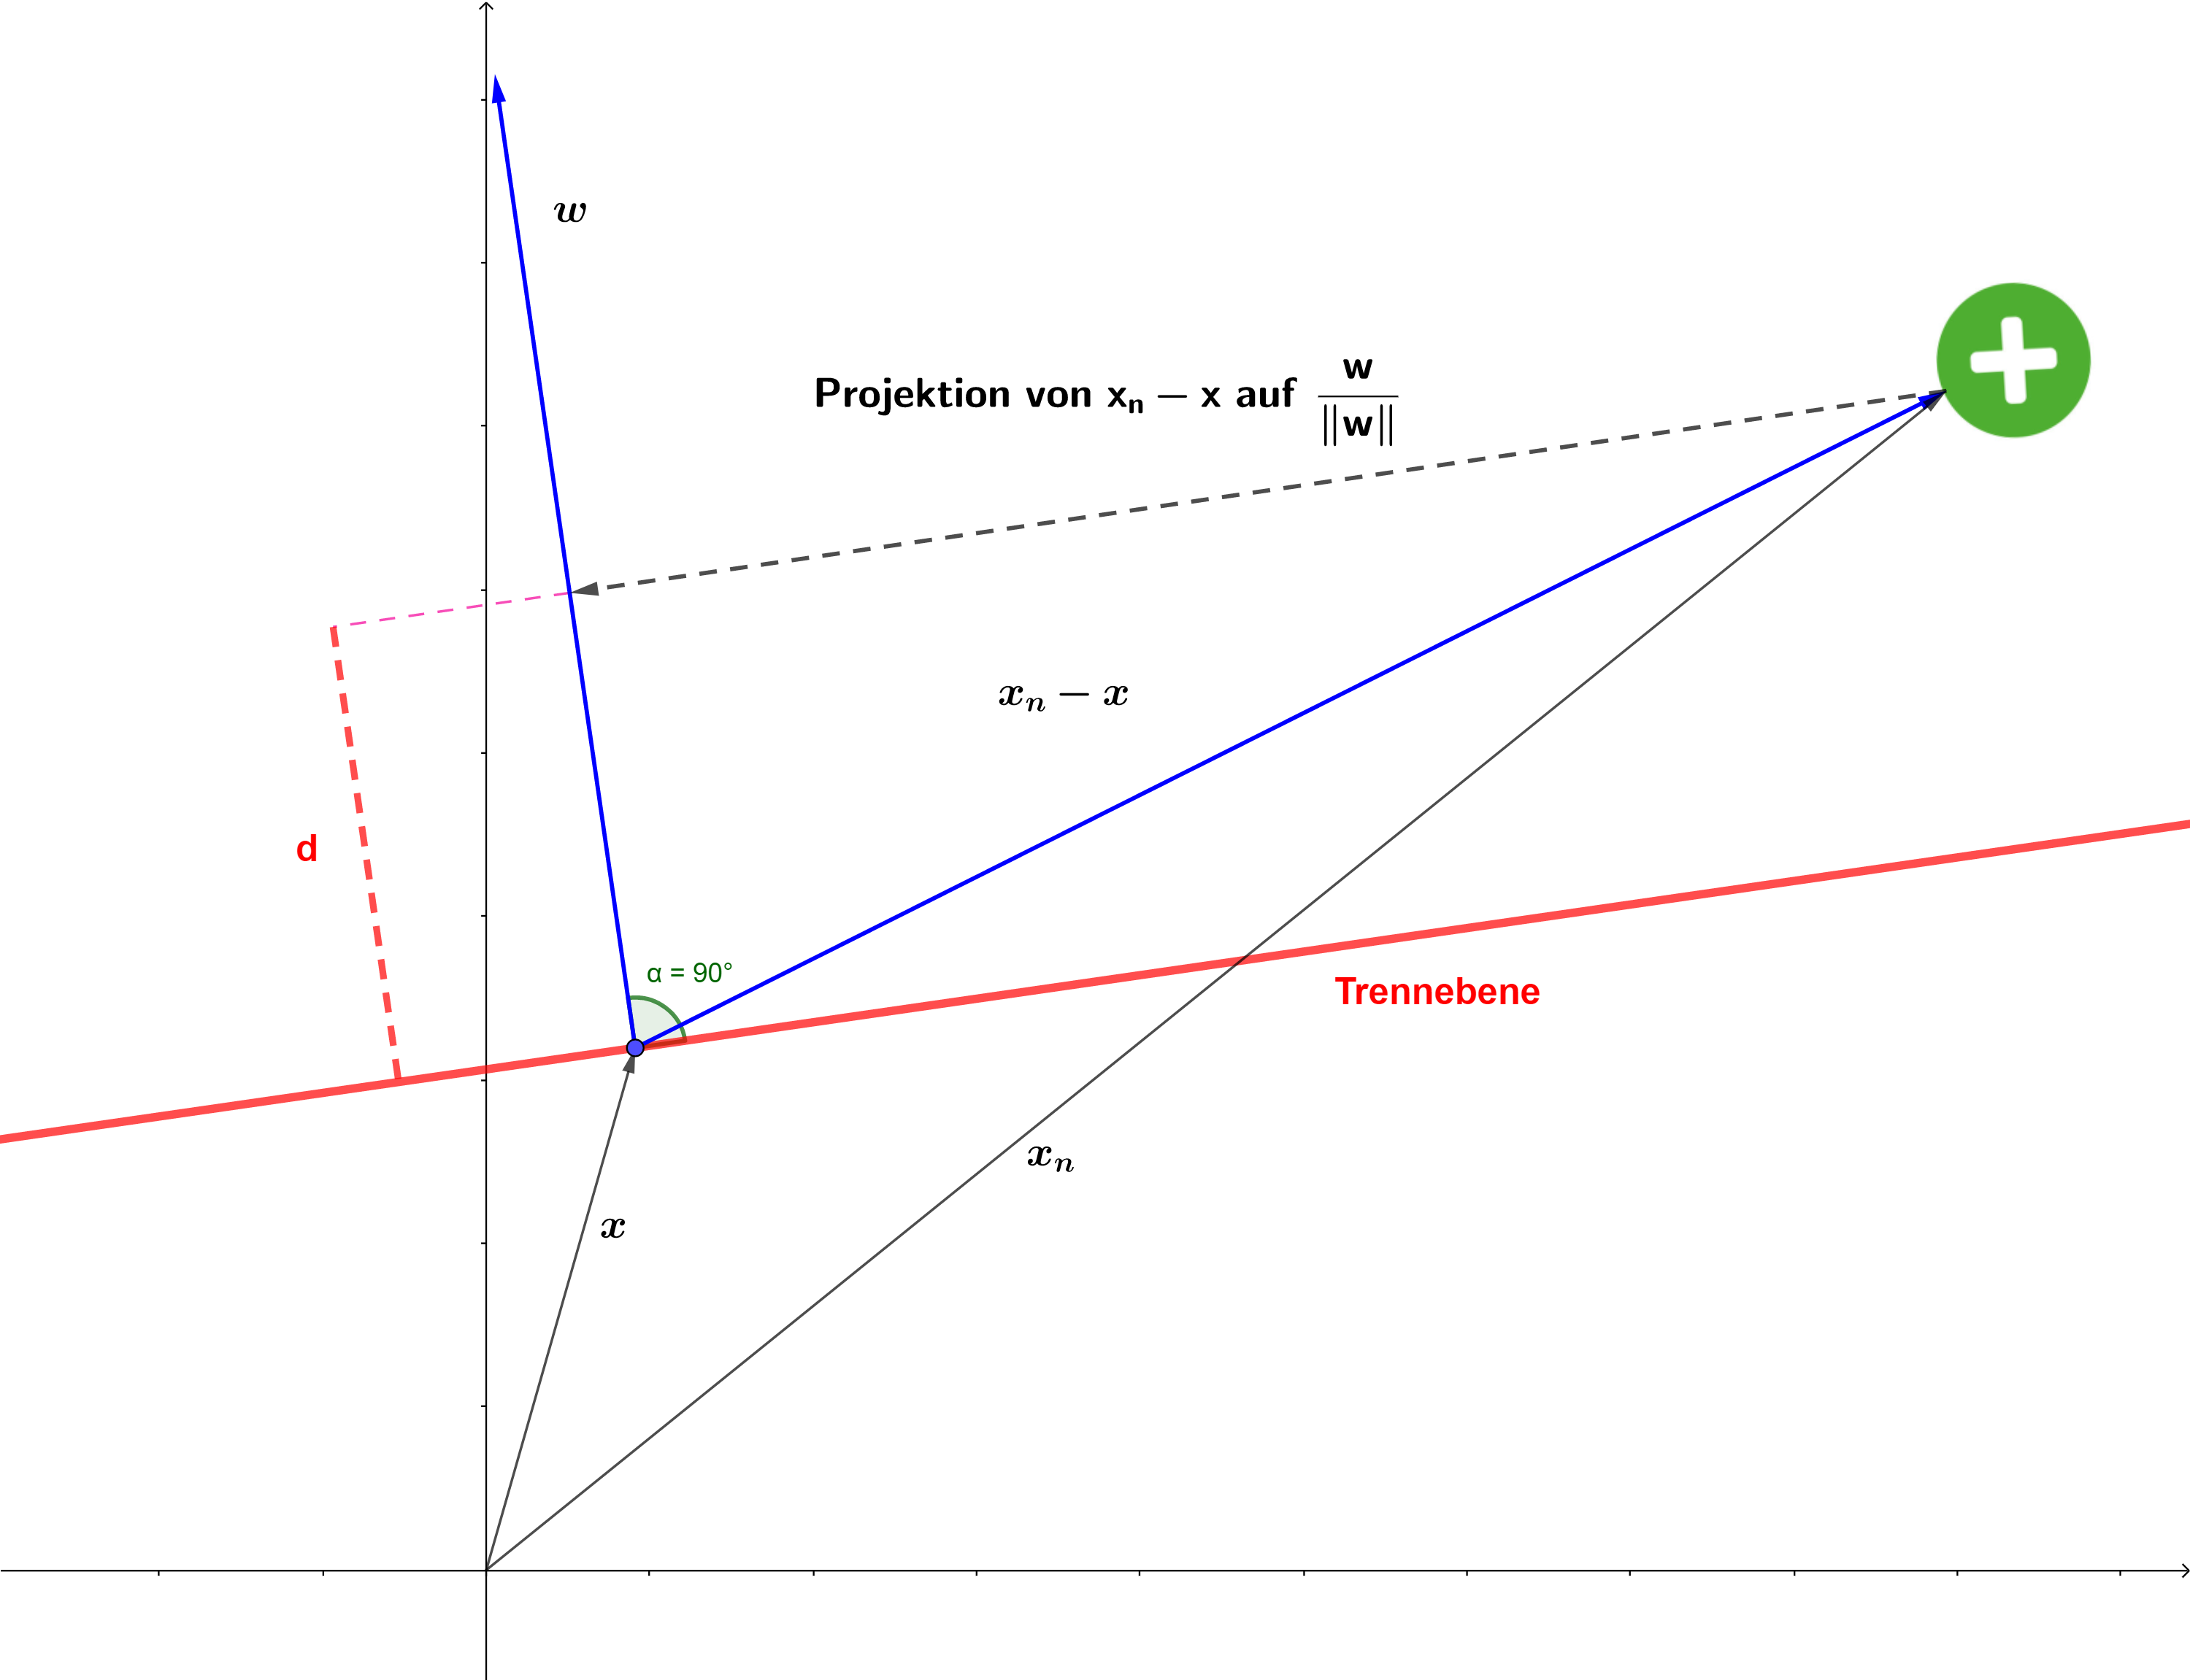
\includegraphics[width=\textwidth,height=0.5\textheight,keepaspectratio]{assets/projection.png}
		\end{figure}
	\end{center}

\end{frame}


\begin{frame}{Normalabstand eines Punktes zur Ebene}
	\begin{equation*}
		\begin{aligned}
			d &= \frac{1}{\norm{w}} | (w^{T} x_{n} + b - (w^{T} x + b)) |
		\end{aligned}
	\end{equation*}

	Weil der Punkt $x$ auf der Ebene liegt gilt $w^{T} x + b = 0$ und somit für den Normalabstand eines beliebigen Punktes $x_{n}$:
	
	\begin{equation*}
		\begin{aligned}
			d &= \frac{1}{\norm{w}} | (w^{T} x_{n} + b) |
		\end{aligned}
	\end{equation*}
\end{frame}


\begin{frame}{Breite des Trennbands}
	
	\begin{equation*}
		\begin{aligned}
			d &= \frac{1}{\norm{w}} | (w^{T} x_{n} + b) |
		\end{aligned}
	\end{equation*}

	Annahme: $x_{n} = \hat{x}$ ist der am nächsten zur Ebene liegende Punkt auf der Grenze des Trennbands\\
	Weil $y_{n} (w^{T} \hat{x} + b) = 1 = |w^{T} \hat{x} + b|$ gilt ergibt sich der minimale Normalabstand $D$: \\
	
	\begin{equation*}
		\begin{aligned}
			D &= \frac{1}{\norm{w}}
		\end{aligned}
	\end{equation*}

	 Weil $D$ der minimale Normalabstand zur Ebene ist, ist $2D$ die Breite des freien Trennbands.

\end{frame}


\begin{frame}{Reminder}
	
	Ziel: lineare Trennung mit möglichst breitem, freien Trennband \\
	
	Entspricht Maximierung:
	\begin{equation*}
		\begin{aligned}
			\max_{w} (2 D) &= \max_{w} \frac{2}{\norm{w}} = \max_{w} \frac{1}{\norm{w}}
		\end{aligned}
	\end{equation*}
	
	\begin{center}
		\begin{figure}
			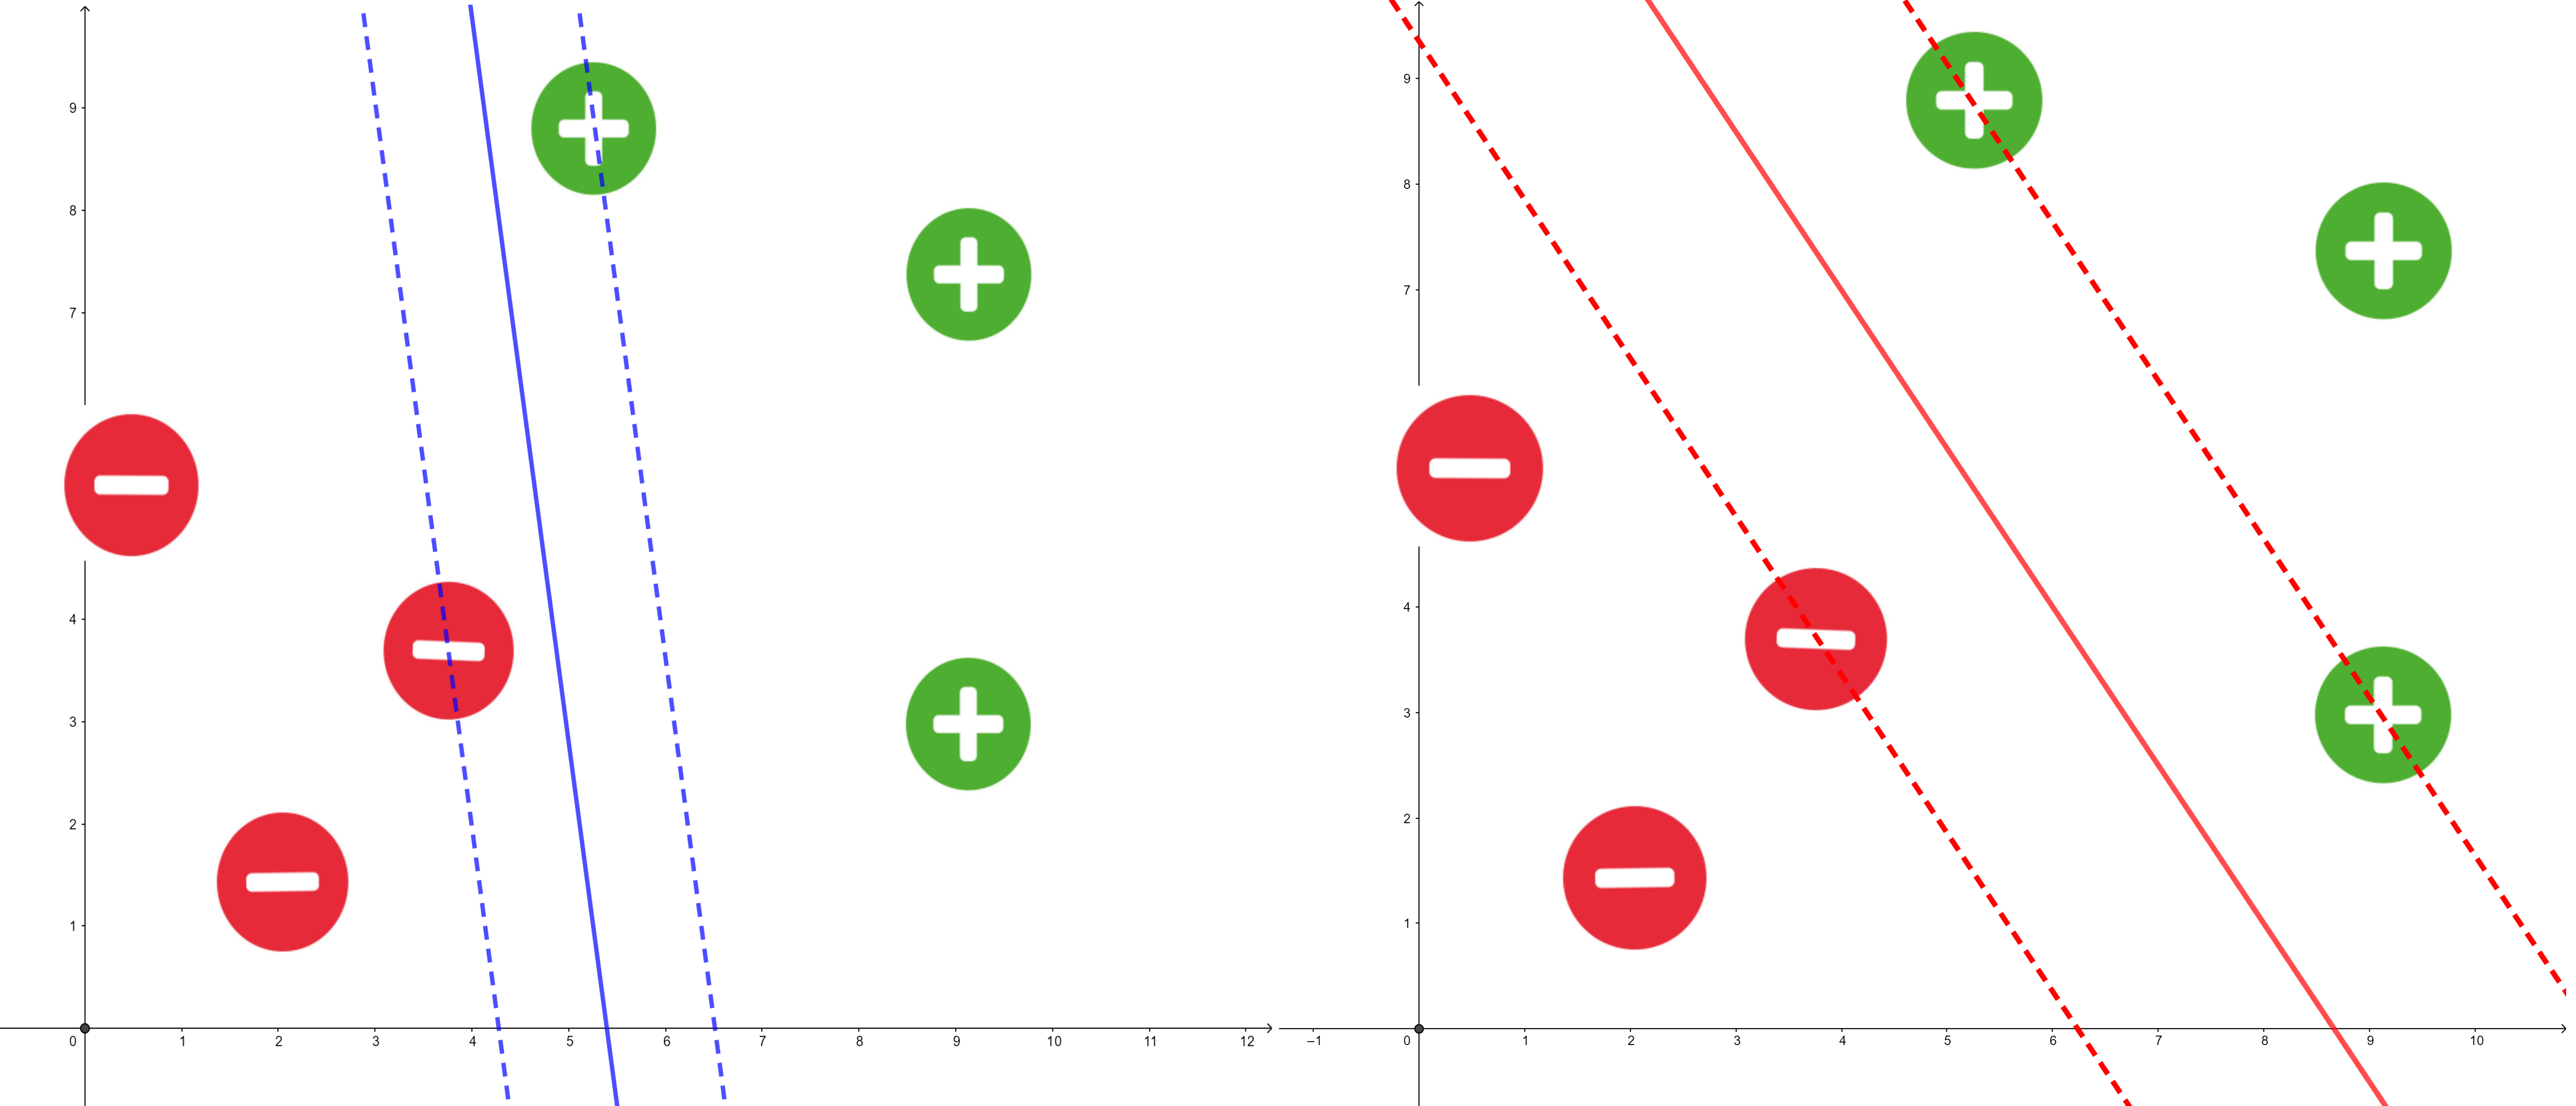
\includegraphics[width=\textwidth,height=0.7\textheight,keepaspectratio]{assets/small_vs_big_margin.png}
		\end{figure}
	\end{center}	
\end{frame}


\begin{frame}{Optimierungsproblem}
	
\begin{subequations}
	\begin{alignat*}{2}
		&\!\max_{w}        &\qquad&  \frac{1}{\norm{w}} \\
		&\text{mit } &      & \min_{n=1..N} |w^{T} x_{n} + b| = 1
	\end{alignat*}
\end{subequations}

\begin{equation*}
	\begin{aligned}
		\min_{n=1..N} |w^{T} x_{n} + b| = 1 \text{  ist der am nächsten zur Ebene liegende Punkt } \hat{x}
	\end{aligned}
\end{equation*}



Beidseitige Multiplikation mit $y_{n}$ zur Vermeidung des Betrags:
\begin{equation*}
	\begin{aligned}
		|w^{T} x_{n} + b| &= y_{n} (w^{T} x_{n} + b)
	\end{aligned}
\end{equation*}
	
\end{frame}


\begin{frame}{Optimierungsproblem}
	Nach Umformung (Maximierung in Minimierung) und Verallgemeinerung der Nebenbedingung auf beliebige Punkte $x_{n}$:
	\begin{subequations}
		\begin{alignat*}{2}
			&\!\min_{w}        &\qquad&  \frac{1}{2} w^{T} w \\
			&\text{mit } &      & y_n (w^{T} x_{n} + b) \geq 1 \text{ für } n=1..N 
		\end{alignat*}
	\end{subequations}

	Bemerkungen:
	\begin{itemize}
		\item Faktor $\frac{1}{2}$ wird so gewählt weil dieser später wegfällt
		\item $w^{T} w $ und $\norm{w}$ sind aus Optimierungssicht gleichbedeutend, Problem ist in dieser Form aber besser optimierbar
	\end{itemize}

\end{frame}

\begin{frame}{Lagrange Optimierung}
	Optimierungsproblem mit Ungleichung als Nebenbedingung \\
	Umformen der Nebenbedingung:
	\begin{subequations}
		\begin{alignat*}{2}
			&\!\min_{w}        &\qquad&  \frac{1}{2} w^{T} w\\
			&\text{mit } &      & y_n (w^{T} x_{n} + b)-1 \geq 0 \text{ für } n=1..N
		\end{alignat*}
	\end{subequations}
\end{frame}

\begin{frame}{Aufstellen der Lagrange Gleichung}
	Ungleichung wird von zu optimierender Funktion abgezogen und Lagrange Multiplikatoren eingeführt:
	\begin{subequations}
		\begin{alignat*}{2}
			&\!\min_{w, b}        &\qquad&  \Lagr (w, b, \alpha) = \frac{1}{2} w^{T} w - \sum_{n=1}^{N} \alpha_{n} (y_n (w^{T} x_{n} + b)-1)\\
			&\max_{\alpha_{n}} &      & \alpha_{n} \geq 0 \text{ für } n=1..N
		\end{alignat*}
	\end{subequations}

	Lösung durch $0$ setzen der partiellen Ableitungen:
	\begin{equation*}
		\begin{aligned}
			\nabla_{w} \Lagr &\overset{!}{=} \vec{0} \\
			\frac{\partial}{\partial b} \Lagr &\overset{!}{=} 0 \\
		\end{aligned}
	\end{equation*}
	
\end{frame}

\begin{frame}{Lösen der Lagrange Gleichung}

	Nach $w$:
	\begin{equation*}
		\begin{aligned}
			\nabla_{w} \Lagr &= w - \sum_{n=1}^{N} \alpha_{n} y_{n} x_{n} \overset{!}{=} \vec{0} \\
			w &= \sum_{n=1}^{N} \alpha_{n} y_{n} x_{n}
		\end{aligned}
	\end{equation*}

	Nach $b$:
	\begin{equation*}
		\begin{aligned}
			\frac{\partial}{\partial b} \Lagr &= - \sum_{n=1}^{N} \alpha_{n} y_{n} \overset{!}{=} 0 \\
			\sum_{n=1}^{N} \alpha_{n} y_{n} &= 0
		\end{aligned}
	\end{equation*}
\end{frame}

\begin{frame}{Rücksubstitution in Lagrange Gleichung}
Aufteilen der Summe:
\begin{equation*}
	\begin{aligned}
		\Lagr(w, b, \alpha) &= \frac{1}{2} w^{T} w - \sum_{n=1}^{N} \alpha_{n} (y_n (w^{T} x_{n} + b)-1) = \\
		&= \frac{1}{2} w^{T} w - [\sum_{n=1}^{N} \alpha_{n} y_{n} b - \sum_{n=1}^{N} \alpha_{n} + \sum_{n=1}^{N} \alpha_{n} y_{n} w^{T} x_{n}]
	\end{aligned}
\end{equation*}

Aus Ableitung nach $b$ wissen wir $\sum_{n=1}^{N} \alpha_{n} y_{n} = 0$:

\begin{equation*}
	\begin{aligned}
		\Lagr(w, b, \alpha) &= \frac{1}{2} w^{T} w - [-\sum_{n=1}^{N} \alpha_{n} + \sum_{n=1}^{N} \alpha_{n} y_{n} w^{T} x_{n}]
	\end{aligned}
\end{equation*}

\end{frame}


\begin{frame}{Rücksubstitution in Lagrange Gleichung}
Vergleicht man den Term $\sum_{n=1}^{N} \alpha_{n} y_{n} w^{T} x_{n}$ mit dem Ergebnis der partiellen Ableitung nach $w$ ($w = \sum_{n=1}^{N} \alpha_{n} y_{n} x_{n}$) erkennt man, dass gilt:

\begin{equation*}
	\begin{aligned}
		\sum_{n=1}^{N} \alpha_{n} y_{n} w^{T} x_{n} &= w^T w = \\
		&= \sum_{n=1}^{N} \sum_{m=1}^{M} y_{n} y_{m} \alpha_{n} \alpha_{m} x_{n}^{T} x_{m}
	\end{aligned}
\end{equation*}

Eingesetzt in Lagrange Gleichung:
\begin{equation*}
	\begin{aligned}
		\Lagr(\alpha) &= \sum_{n=1}^{N }\alpha_{n} - \frac{1}{2} \sum_{n=1}^{N} \sum_{m=1}^{M} y_{n} y_{m} \alpha_{n} \alpha_{m} x_{n}^{T} x_{m}
	\end{aligned}
\end{equation*}

\end{frame}


\begin{frame}{Maximierung ohne Nebenbedingung}
	Quadratic Programming Problem ($x_{n}^{T} x_{m}$):
	\begin{subequations}
		\begin{alignat*}{2}
			&\!\max_{\alpha}        &\qquad&  	\Lagr(\alpha) = \sum_{n=1}^{N} \alpha_{n} - \frac{1}{2} \sum_{n=1}^{N} \sum_{m=1}^{M} y_{n} y_{m} \alpha_{n} \alpha_{m} x_{n}^{T} x_{m}\\
			&\text{mit } &      & \alpha_{n} \geq 0 \text{ für } n=1..N \\
			&       & & \sum_{n=1}^{N} \alpha_{n} y_{n} = 0\text{ für } n=1..N
		\end{alignat*}
	\end{subequations}

	Lösung mittels QP-Solver \\
	Ergebnis: $\alpha$ Vektor mit $\alpha_{n}$ Lagrange-Multiplikatoren

\end{frame}


\begin{frame}{Schlupfterm}
	Reminder Ausgangsproblem:
	\begin{subequations}
		\begin{alignat*}{2}
			&\!\min_{w, b}        &\qquad&  \Lagr (w, b, \alpha) = \frac{1}{2} w^{T} w - \sum_{n=1}^{N} \alpha_{n} (y_n (w^{T} x_{n} + b)-1)\\
			&\max_{\alpha_{n}} &      & \alpha_{n} \geq 0 \text{ für } n=1..N
		\end{alignat*}
	\end{subequations}
	
	
	 $\alpha_{n} (y_n (w^{T} x_{n} + b)-1)$ (\glqq Schlupf \grqq) wird $0$ wenn:
	 \begin{itemize}
	 	\item $\alpha_{n} = 0$ oder 
	 	\item $(y_n (w^{T} x_{n} + b)-1) = 0$
	 \end{itemize}
	 
	 Umgekehrt: Alle $x_{n}$ mit $\alpha_{n} \neq 0$ haben Schlupf $0$, liegen also am nächsten zur Trennebene. \\
	 
	 Diese Vektoren werden \textbf{Stützvektoren} genannt.
\end{frame}

\begin{frame}{Bestimmung Gewichtsvektor}
	
	$\alpha$ Vektor mit $\alpha_{n}$ Faktoren ist bekannt aus QP-Solver\\
	Viele $\alpha_{i}$ werden $0$ sein, die $\alpha_{i} \neq 0$ gehören zu den Stützvektoren $x_{i}$. \\
	Damit kann Formel für $w$
	\begin{equation*}
		\begin{aligned}
			w &= \sum_{n=1}^{N} \alpha_{n} y_{n} x_{n}
		\end{aligned}
	\end{equation*}

	vereinfacht werden:
	\begin{equation*}
	\begin{aligned}
		w &= \sum_{n \text{ ist Stützvektor}} \alpha_{n} y_{n} x_{n}
	\end{aligned}
	\end{equation*}

	Die Bezeichnung Stützvektor ergibt sich, weil die Ebene durch diese Vektoren \glqq gestützt \grqq wird. Alle Vektoren mit $\alpha_{n} = 0$ haben keinen Einfluss!
\end{frame}

\begin{frame}{Bestimmung Bias}
	
	$y_n (w^{T} x_{n} + b) = 1$ gilt für Stützvektoren, daher kann mit beliebigem Stützvektor $x_{n}$ der Bias bestimmt werden:
	
	\begin{equation*}
		\begin{aligned}
			b &= \frac{1}{y_{n}} - w^{T} x_{n} = \\
			&= y_{n} - w^{T} x_{n} 
		\end{aligned}
	\end{equation*}
	
	
\end{frame}


\section{Lösung mittels QP-Solver}

\begin{frame}{Lösung mittels QP-Solver}
	
	Standardform von QP-Problemen:
	\begin{equation*} \label{std_QP_problem}
		\begin{aligned}
			\min_{x} &= \frac{1}{2} x^{T} Q x + c x + d 
		\end{aligned}
	\end{equation*}
	
	Umformung Maximierung in Minimierung weil $\max -f(x) = \min f(x)$:
	\begin{equation*} \label{qp_adapt1}
		\begin{aligned}
			\min_{\alpha} \Lagr(\alpha) &= \frac{1}{2} \sum_{n=1}^{N} \sum_{m=1}^{M} y_{n} y_{m} \alpha_{n} \alpha_{m} x_{n}^{T} x_{m} - \sum_{n=1}^{N} \alpha_{n}
		\end{aligned}
	\end{equation*}
\end{frame}

\begin{frame}{Problem in QP-Standardform}
	
	\begin{equation*}
		\begin{aligned}
			\min_{\alpha} \Lagr(\alpha) &= \frac{1}{2} \sum_{n=1}^{N} \sum_{m=1}^{M} y_{n} y_{m} \alpha_{n} \alpha_{m} x_{n}^{T} x_{m} - \sum_{n=1}^{N} \alpha_{n}
		\end{aligned}
	\end{equation*}
	
	In QP-Standardform $\rightarrow$ Lösungs-Frameworks:
	
	\begin{subequations}
		\begin{alignat*}{2}
			&\!\min_{\alpha}        &\qquad& \Lagr(\alpha) = \frac{1}{2} \alpha^{T} Q \alpha + (-1^T) \alpha \label{eq:qp1}\\
			&\text{mit} &      & Q = \begin{bmatrix} 
				y_{1}y_{1}x_{1}^{T}x_{1} & y_{1}y_{2}x_{1}^{T}x_{2} & \dots & y_{1}y_{N}x_{1}^{T}x_{N}\\
				y_{2}y_{1}x_{2}^{T}x_{1} & y_{2}y_{2}x_{2}^{T}x_{2} & \dots & y_{2}y_{N}x_{2}^{T}x_{N}\\
				\vdots & \vdots & \vdots & \vdots\\
				y_{N}y_{1}x_{N}^{T}x_{1} & y_{N}y_{2}x_{N}^{T}x_{2} & \dots & y_{N}y_{N}x_{N}^{T}x_{N}\\ 
			\end{bmatrix}
		\end{alignat*}
	\end{subequations}

	\pause

	$Q$ ist $N \times N$ Matrix. Problematisch bei großen Trainingssets!
\end{frame}

\begin{frame}{Lösung mittels QP-Solver}
	Ergebnis des QP-Solvers: $\alpha = (\alpha_{1}, \alpha_{2}, ..., \alpha_{n})$ \\
	
	Berechnung von $w$ und $b$ wie zuvor gezeigt:
	
	\begin{equation*}
		\begin{aligned}
			w &= \sum_{n=1}^{N} \alpha_{n} y_{n} x_{n}
		\end{aligned}
	\end{equation*}

	Mit beliebigem Stützvektor $x_{k}$:
	\begin{equation*}
		\begin{aligned}
			b &= \frac{1}{y_{k}} - w^{T} x_{k}
		\end{aligned}
	\end{equation*}

	Klassifikation neuer Eingaben $x$:
	\begin{equation*}
		\begin{aligned}
			y &= sign(w^{T} x + b)
		\end{aligned}
	\end{equation*}

\end{frame}

\section{Soft-Margin Support Vector Machine}

\begin{frame}{Einführung Soft-Margin SVM}
	Annahme bisher: Daten linear trennbar ohne Fehler \\
	
	\begin{center}
		\begin{figure}
			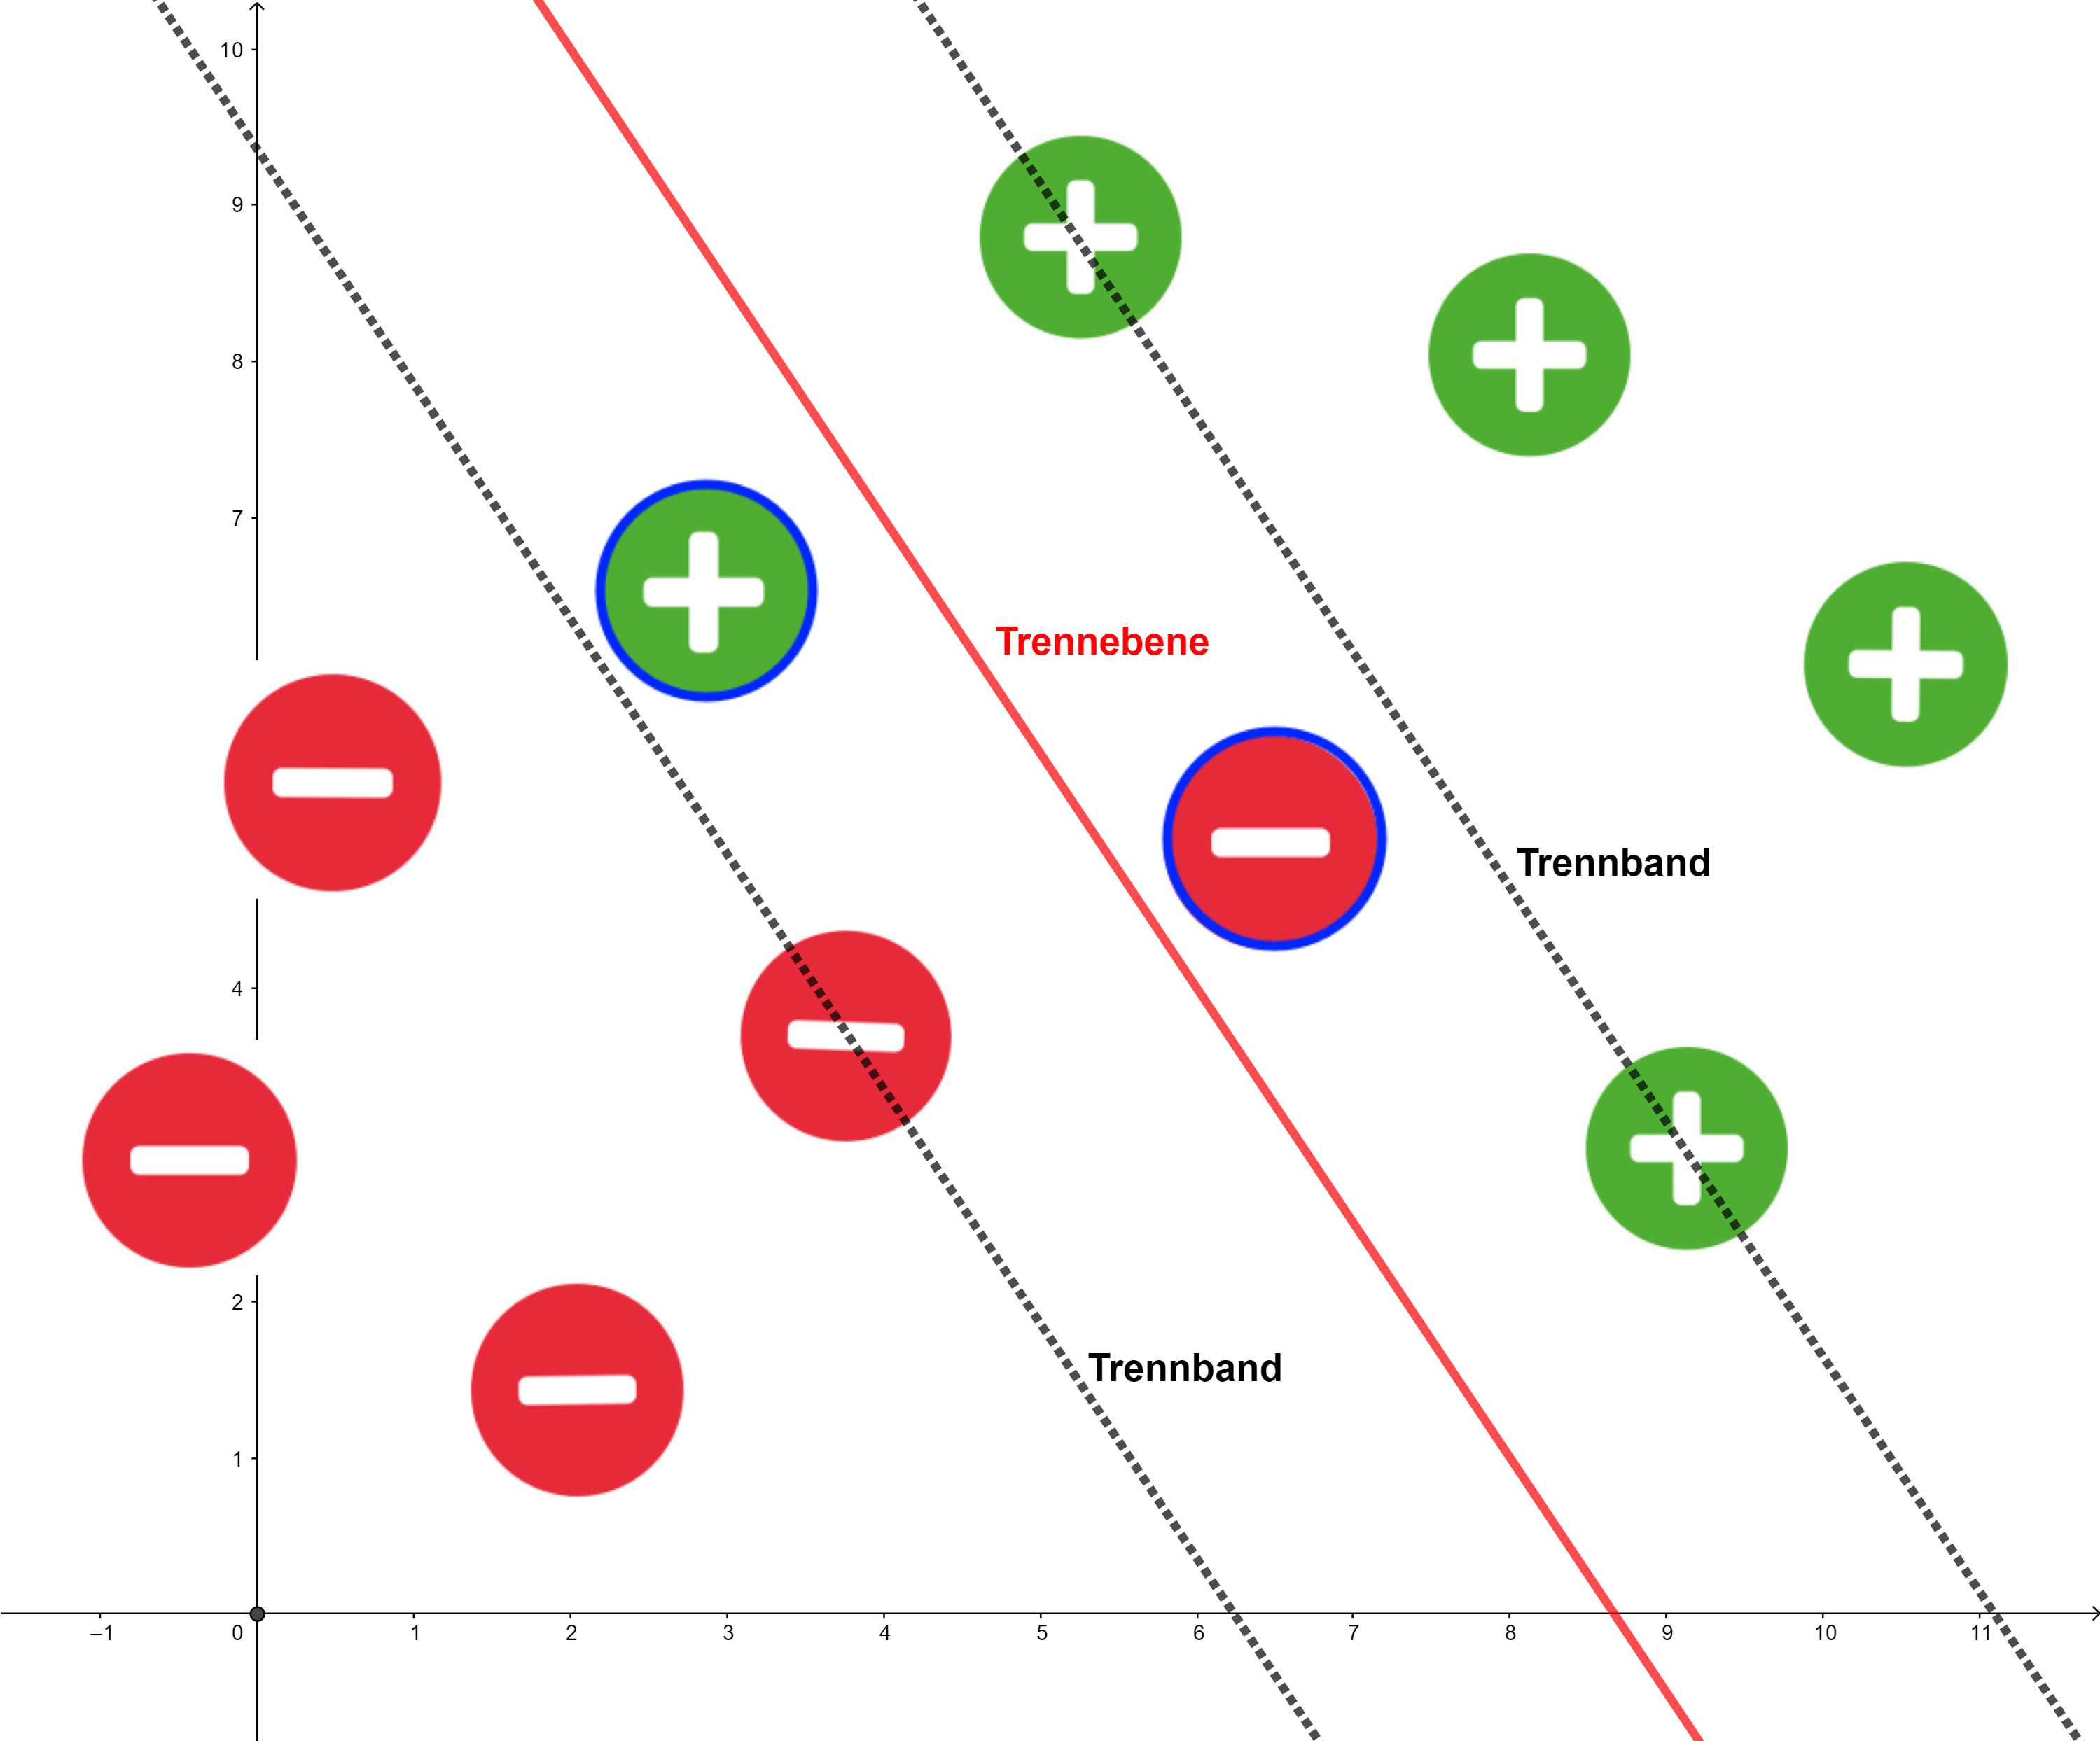
\includegraphics[width=\textwidth,height=0.7\textheight,keepaspectratio]{assets/soft_margin_example.png}
		\end{figure}
	\end{center}
\end{frame}

\begin{frame}{Einführung von Fehlervariablen}
	Problem: bisheriger Algorithmus terminiert nicht bei Fehlern \\
	Lösung: Einführung von positiven Fehlervariablen $\xi_{n} \in \mathbb{R}^{K}, \xi_{n} \geq 0$:
	
	\begin{subequations}
		\begin{alignat*}{2}
			w^{T} x_{n} + b \geq +1 - \xi_{n}& \qquad & \text{ für } y_{n} = +1\\
			w^{T} x_{n} + b \leq -1 + \xi_{n}& & \text{ für } y_{n} = -1
		\end{alignat*}
	\end{subequations}

	Wann kann einzelne Fehlklassifikation auftreten? Wenn $\xi_{n} > 1$ \\
	
	Obere Grenze Anzahl Fehler:
	\begin{equation*}
		\begin{aligned}
			E = C(\sum_{n=1}^{N} \xi_{n})
		\end{aligned}
	\end{equation*}

	$C \in \mathbb{R}, C \geq 0$: \glqq Straffaktor\grqq für Fehler
\end{frame}

\begin{frame}{Erweiterung Optimierungsproblem um Fehlerterm}
	Ziel: Optimales $w$ mit möglichst wenig Fehlern:
	\begin{subequations}
		\begin{alignat*}{2}
			&\!\min_{w}        &\qquad&  \frac{1}{2} w^{T} w + C(\sum_{n=1}^{N} \xi_{n})\\
			&\text{mit } &      & y_n (w^{T} x_{n} + b)-1 \geq 0 \text{ für } n=1..N
		\end{alignat*}
	\end{subequations}

	Ableiten, $0$ setzen und lösen wie zuvor... \\
	
\end{frame}

\begin{frame}{Soft-Margin SVM Optimierungsproblem}
	Soft-Margin Optimierungsproblem:
	\begin{subequations}
		\begin{alignat*}{2}
			&\!\max_{\alpha}        &\qquad&  	\Lagr(\alpha) = \sum_{n=1}^{N} \alpha_{n} - \frac{1}{2} \sum_{n=1}^{N} \sum_{m=1}^{M} y_{n} y_{m} \alpha_{n} \alpha_{m} x_{n}^{T} x_{m} \\
			&\text{mit } &      & 0 \leq \alpha_{n} \leq C \text{ für } n=1..N\\
			&       & & \sum_{n=1}^{N} \alpha_{n} y_{n} = 0\text{ für } n=1..N
		\end{alignat*}
	\end{subequations}

	Einziger Unterschied zu Hard-Margin: Beschränkung $\alpha_{n} \leq C$ (Hard-Margin: $\alpha_{n} \leq \infty$)\\
	
	\pause
	
	Umgekehrt: Soft-Margin mit $C \rightarrow \infty$ entspricht Hard-Margin \\

	Lösung: Wie zuvor gezeigt mit QP-Solver
\end{frame}



\section{Vergleich Hard- \& Soft-Margin Support Vector Machine}

\begin{frame}{Vergleich Hard- \& Soft-Margin SVM}
	Hard-Margin: einzelne Ausreißer bestimmen Lage der Ebene
	Soft-Margin: Fehlklassifikationen zugunsten besserer Gesamt-Trennung
	
	\begin{center}
		\begin{figure}
			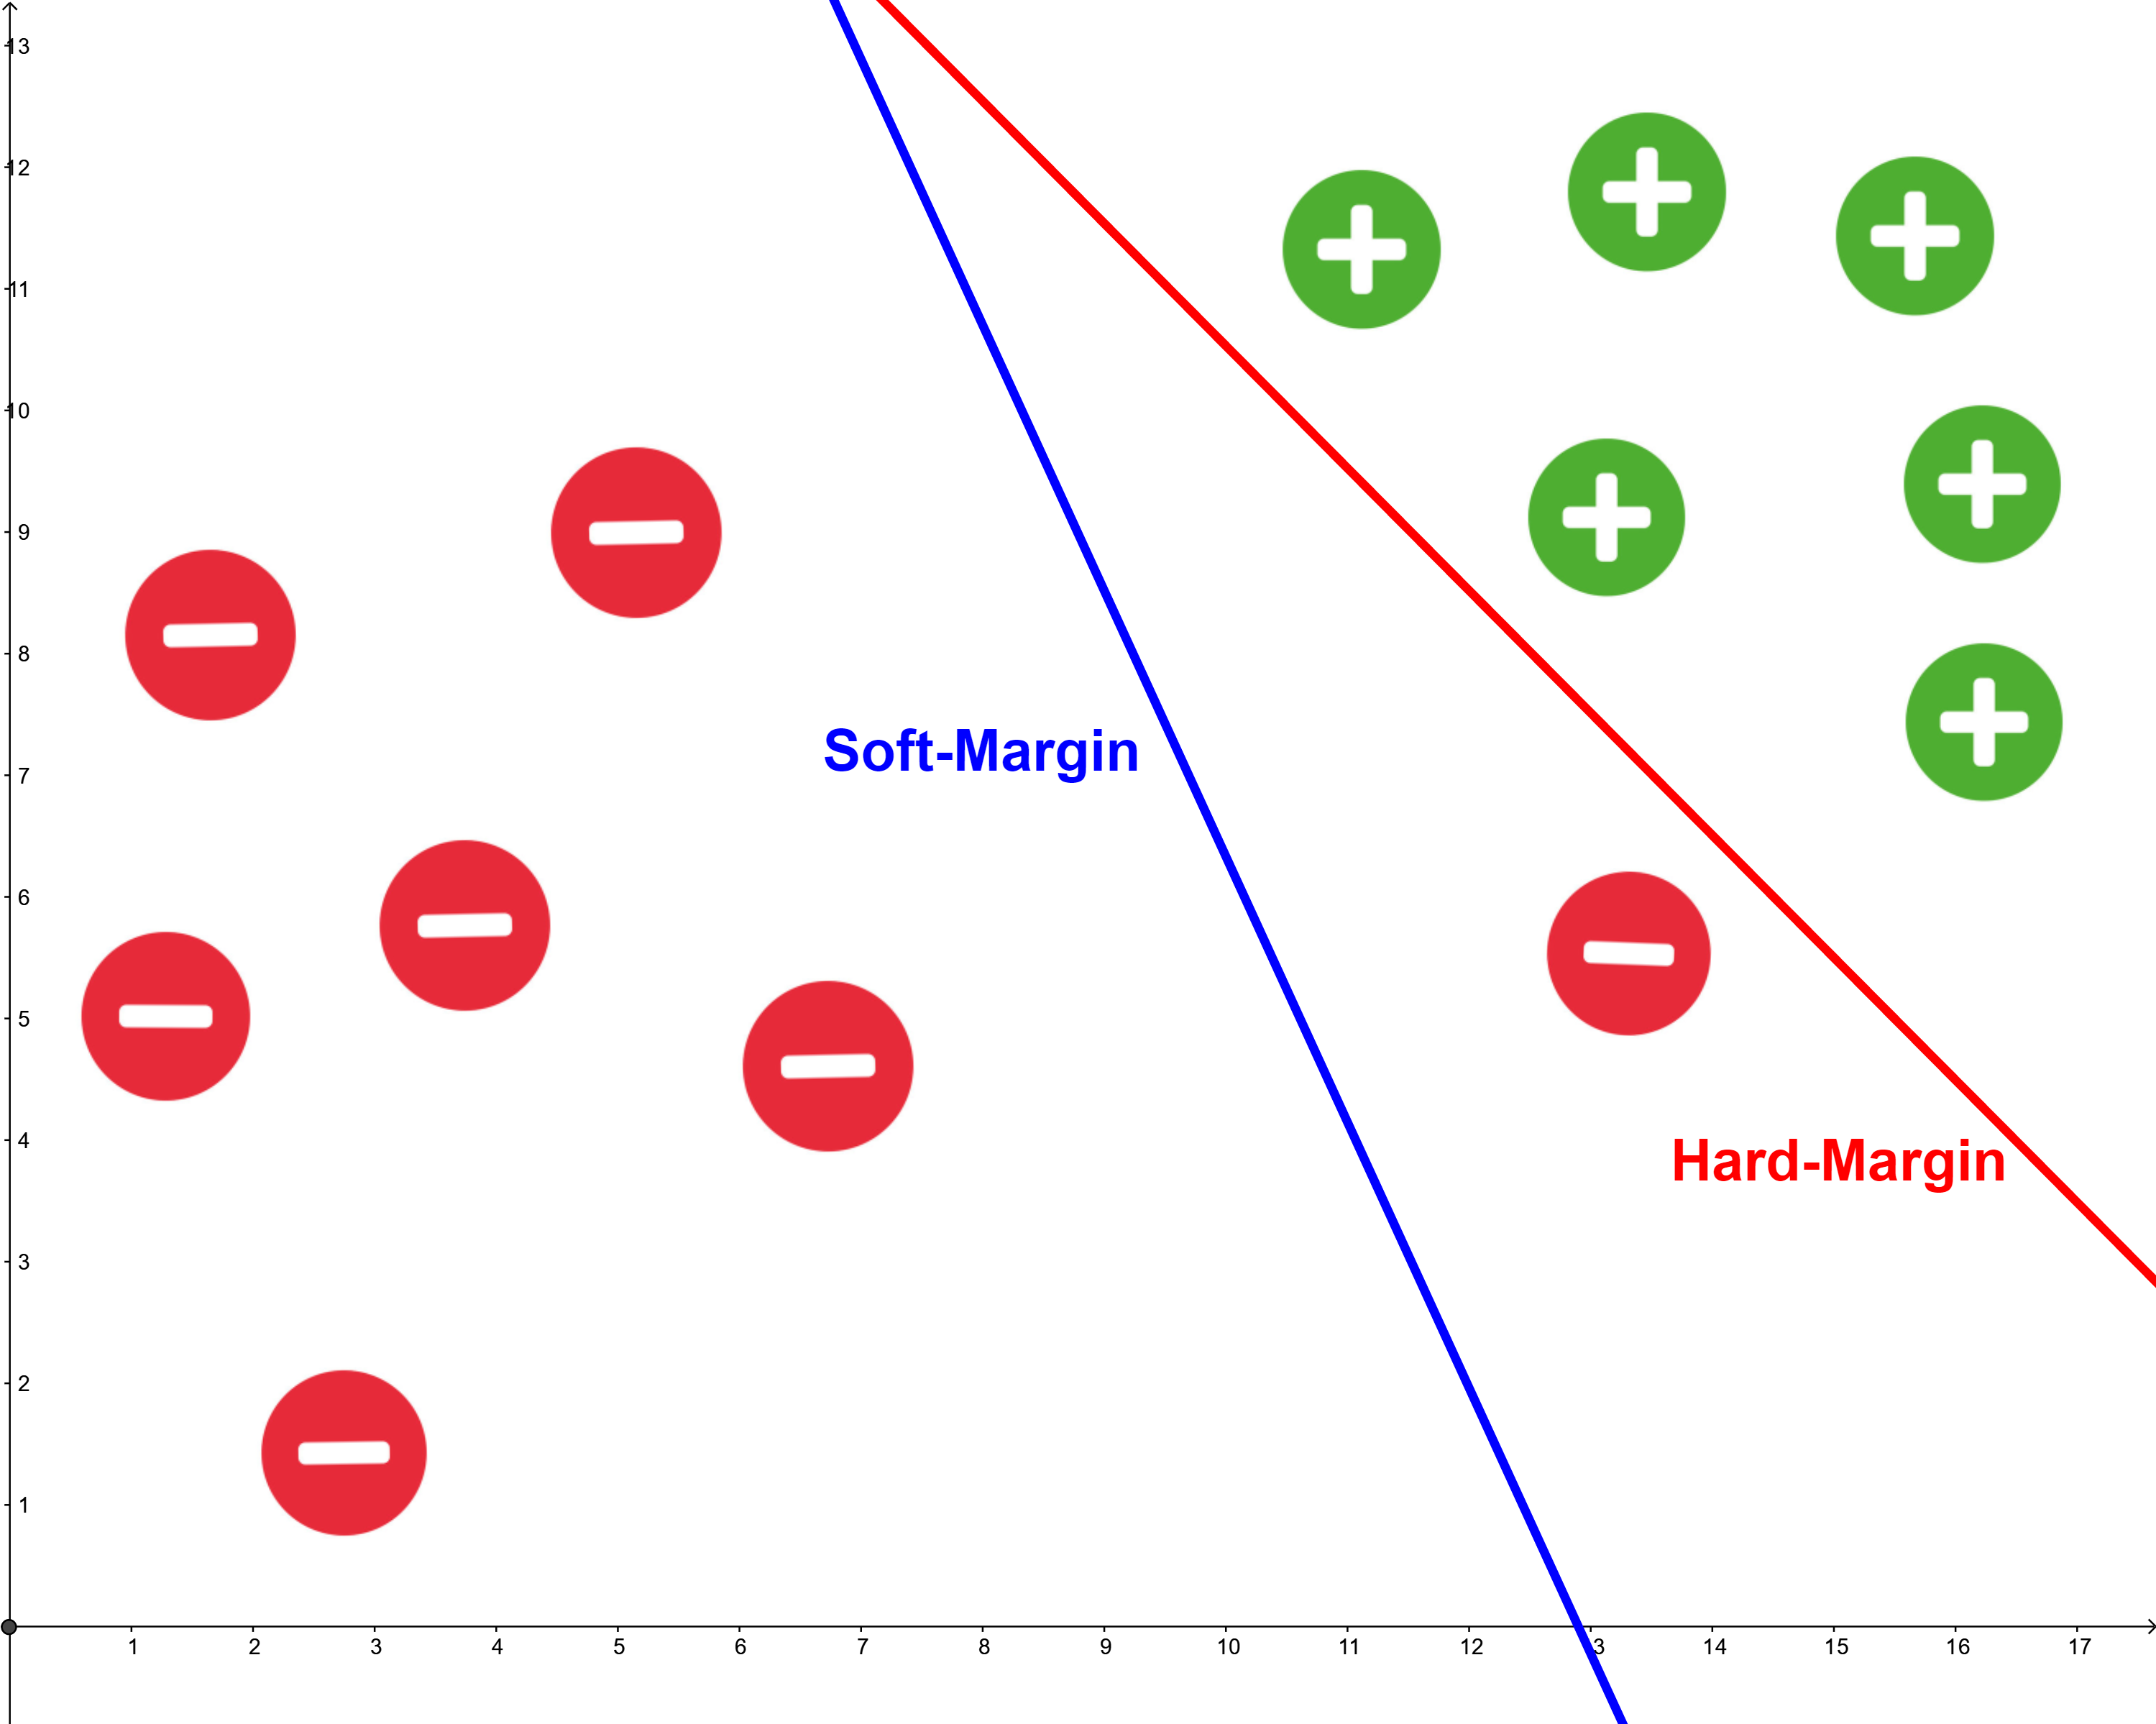
\includegraphics[width=\textwidth,height=0.7\textheight,keepaspectratio]{assets/hard_vs_soft_margin.png}
		\end{figure}
	\end{center}
	
\end{frame}



\section{Nichtlineare Trennung}\label{sec:nichtlintrenn}
\begin{frame}{Einleitung}
    \emph{Ziel}: nichtlineare Trennung \\
    \emph{Problem}: SVM trennt ausschließlich linear \\ \pause
    \emph{Lösung}: Transformation Eingabevektoren in linear trennbaren Raum \\
    Transformationsfunktion $\Phi(x): \mathbb{R}^{K} \rightarrow \mathbb{R}^{L}$ \\
    \begin{center}
        \begin{figure}
            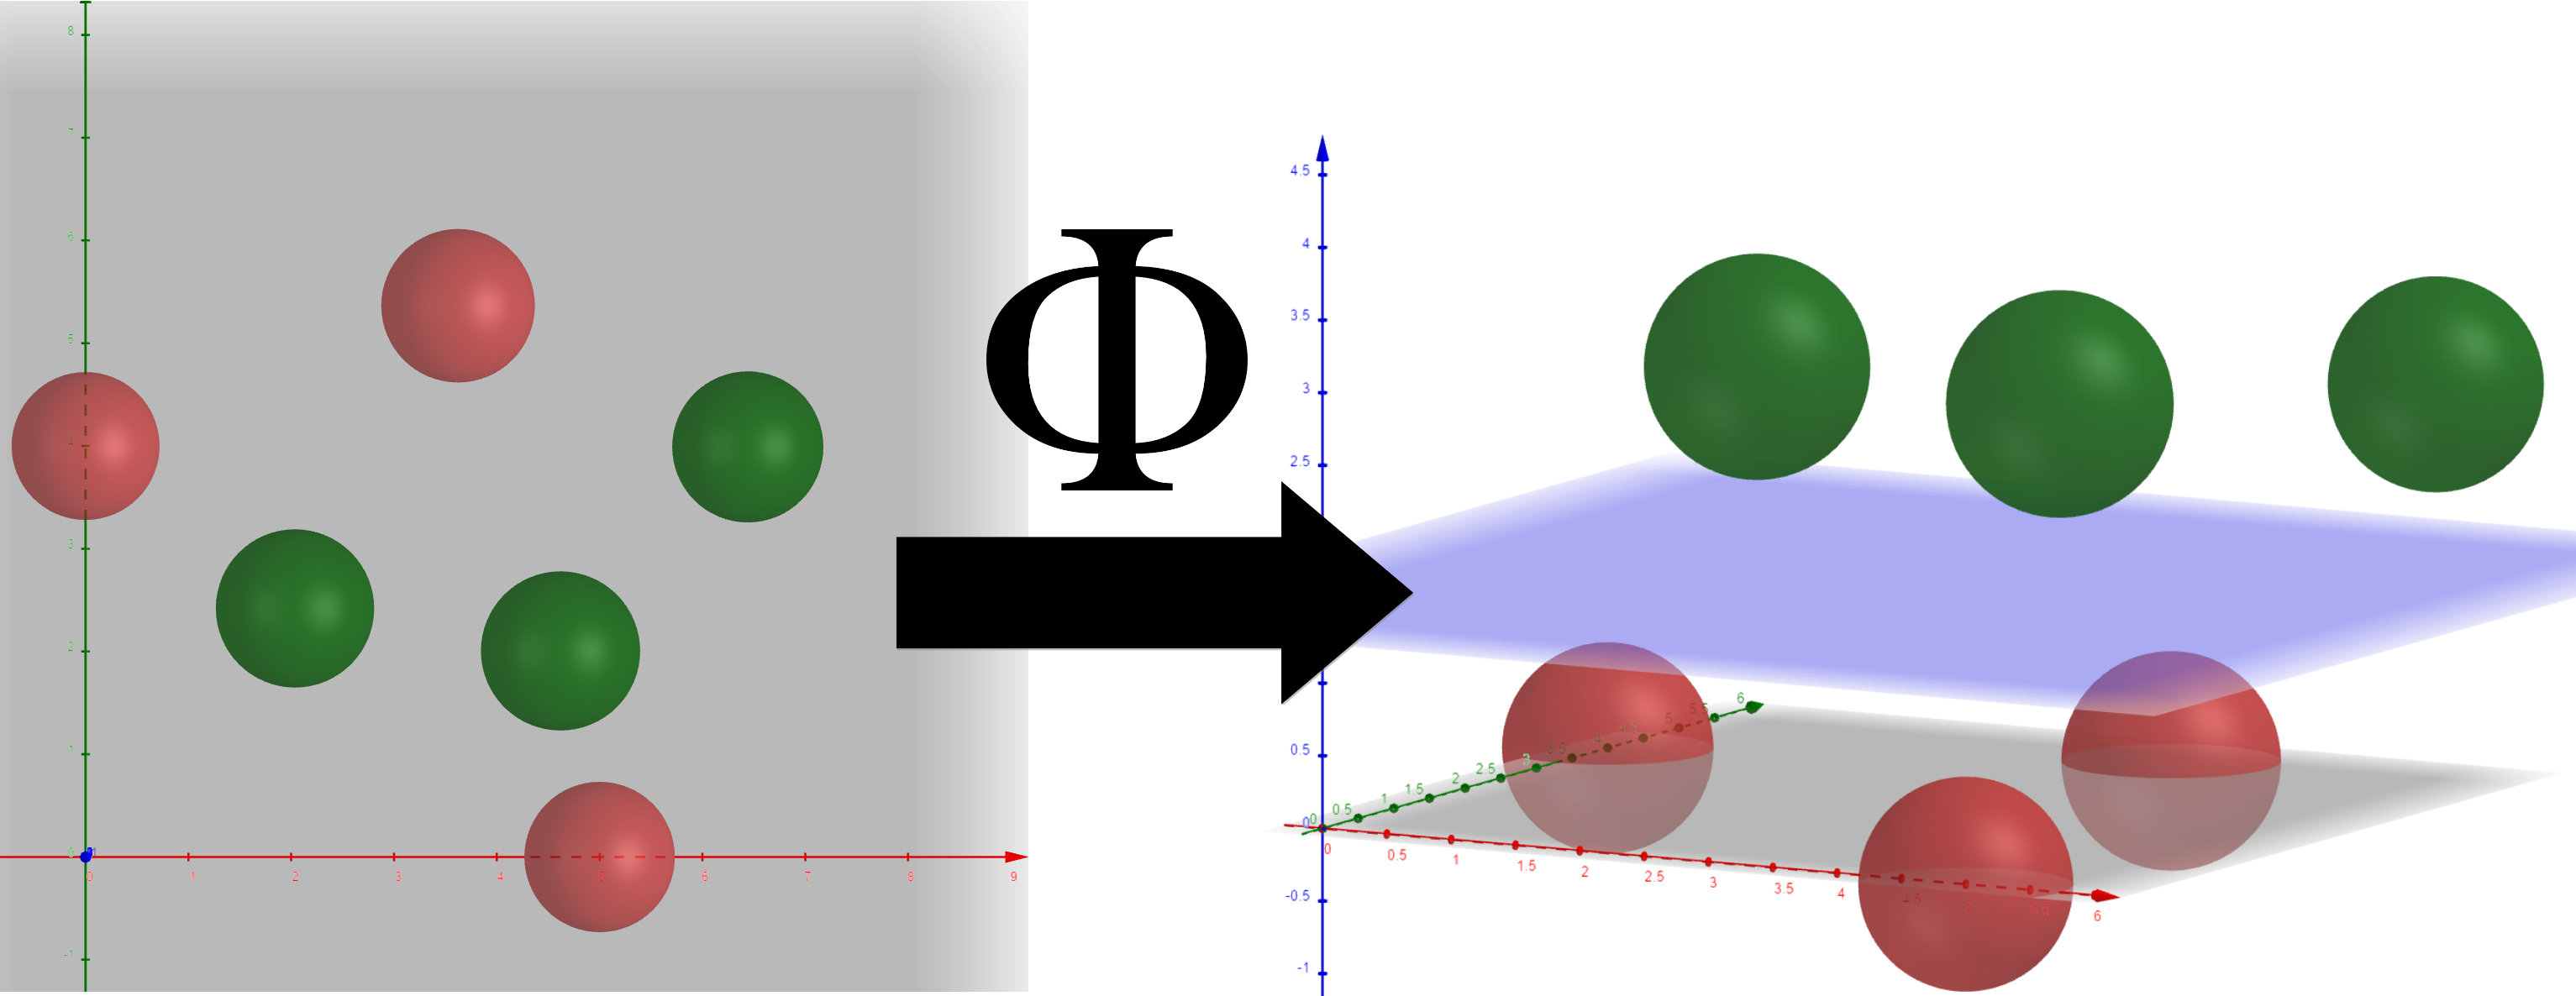
\includegraphics[width=\textwidth,height=0.7\textheight,keepaspectratio]{assets/2d_to_3d_phi}
            \caption{Transformation Eingabevektoren macht linear trennbar}
            \label{fig:transmachtlinear}
        \end{figure}
    \end{center}
\end{frame}

\begin{frame}{Optimierungsproblem transformiert}
Optimierungsproblem mit transformierten Eingabevektoren: \\ \pause
\begin{subequations} \label{eq:soft_margin_with_transform_pres}
\begin{alignat*}{2}
    &\!\max_{\alpha}        &\qquad&  	\Lagr(\alpha) = \sum_{n=1}^{N} \alpha_{n} - \frac{1}{2} \sum_{n=1}^{N} \sum_{m=1}^{M} y_{n} y_{m} \alpha_{n} \alpha_{m} \Phi(x_{n})^{T} \Phi(x_{m})\\
    &\text{mit } &      & 0 \leq \alpha_{n} \leq C \text{ für } n=1..N\\
    &       & & \sum_{n=1}^{N} \alpha_{n} y_{n} = 0\text{ für } n=1..N
\end{alignat*}
\end{subequations} \pause
    Anzahl Lagrangefaktoren $\alpha$ und Dimension der $Q$-Matrix hängen von Anzahl Eingabevektoren ab, nicht von der Dimension \\ \pause
    => Zusatzkosten: Berechnung höherdimensionaler Skalarprodukte $\Phi(x)^{T} \Phi(x)$
\end{frame}

\begin{frame}{Probleme und Erkenntnisse}
    \emph{Problem 1}: Wahl der Transformationsfunktion $\Phi(x)$ \\ \pause
    \emph{Problem 2}: Eingabevektoren in sehr hochdimensionalen/unendlichen Raum transformiert -> Berechnung Skalarprodukt sehr aufwändig/unmöglich \\ \pause
    \emph{Erkenntnis 1}: Transformation erlaubt Bestimmung nichtlinearer Trenngrenzen \\ \pause
    \emph{Erkenntnis 2}: Dimension Vektoren beeinflusst Optimierungsproblem nicht stark \\ \pause
    \emph{Verbesserung}: Umgehung Zusatzkosten der transformierten Skalarprodukte => Kernel Trick
\end{frame}

\begin{frame}{Kernel Trick} % TODO: this slide necessary?
    Es gilt: $z = \Phi(x)$ \\
    \begin{subequations}
        \begin{alignat*}{2}
            &\!\max_{\alpha}        &\qquad&  	\Lagr(\alpha) = \sum_{n=1}^{N} \alpha_{n} - \frac{1}{2} \sum_{n=1}^{N} \sum_{m=1}^{M} y_{n} y_{m} \alpha_{n} \alpha_{m} z_{n}^{T} z_{m}\\
            &\text{mit } &      & 0 \leq \alpha_{n} \leq C \text{ für } n=1..N\\
            &       & & \sum_{n=1}^{N} \alpha_{n} y_{n} = 0\text{ für } n=1..N
        \end{alignat*}
    \end{subequations}
    \pause
    Berechnung von $w$ und $b$:
    \begin{equation*}
        \begin{aligned}
            w &= \sum_{n=1}^{N} \alpha_{n} y_{n} z_{n}
        \end{aligned}
    \end{equation*}

    \begin{equation*}
        \begin{aligned}
            b &= \frac{1}{y_{k}} - w^{T} z_{k}
        \end{aligned}
    \end{equation*}
\end{frame}

\begin{frame}{Kernel Trick}
    Einführung einer Kernel-Funktion $K(x, x') = z_{1}^{T} z_{2} = \Phi(x)^{T} \Phi(x')$ \\ \pause
    Berechnet Skalarprodukt der transformierten Eingabevektoren \\
    Transformiert Eingabevektoren aber nicht tatsächlich in den neuen Raum \\ \pause
    Berechnung hochdimensionaler Skalarprodukte wird umgangen
\end{frame}

\begin{frame}{Beispiel Kernel-Funktion}
    Kernel-Funktion für $x, x' \in \mathbb{R}^2$: \\
    \begin{equation*} \label{eq:example1_kernel_pres}
    \begin{aligned}
        K(x, x') &= (1 + x^{T}x')^{2} = \\ \pause
        &= (1 + x_{1} x_{1}' + x_{2} x_{2}')^{2} = \\ \pause
        &= 1 + x_{1}^2 x_{1}'^2 + x_{2}^{2} x_{2}'^{2} + 2x_{1} x_{1}' + 2 x_{2} x_{2}' + 2 x_{1} x_{1}'x_{2} x_{2}'
    \end{aligned}
    \end{equation*}
\end{frame}

\begin{frame}{Beweis Kernel-Funktion entspricht Skalarprodukt}
    Annahme für verwendete Transformationsfunktion $\Phi$: \\
    \begin{equation*}
        \begin{aligned}
            \Phi(x) &= (1, x_{1}^{2}, x_{2}^{2}, \sqrt{2} x_{1}, \sqrt{2} x_{2}, \sqrt{2} x_{1} x_{2})\\
        \end{aligned}
    \end{equation*}
    Anwendung auf Vektoren $x$ und $x'$: \\ \pause
    \begin{equation*} \label{eq:example1_innerprod_pres}
    \begin{aligned}
        \Phi(x) &= (1, x_{1}^{2}, x_{2}^{2}, \sqrt{2} x_{1}, \sqrt{2} x_{2}, \sqrt{2} x_{1} x_{2})\\ \pause
        \Phi(x') &= (1, x_{1}'^{2}, x_{2}'^{2}, \sqrt{2} x_{1}', \sqrt{2} x_{2}', \sqrt{2} x_{1}' x_{2}')\\ \pause
        \Phi(x)^T \Phi(x') &= 1 + x_{1}^2 x_{1}'^2 + x_{2}^{2} x_{2}'^{2} + 2x_{1} x_{1}' + 2 x_{2} x_{2}' + 2 x_{1} x_{1}'x_{2} x_{2}'
    \end{aligned}
    \end{equation*} \pause
    Kernel-Funktion $K(x, x') = (1 + x^{T}x')^{2}$ entspricht Skalarprodukt der mit $\Phi$ transformierten Vektoren $x, x'$
\end{frame}

\begin{frame}{Polynomieller Kernel}
    Verallgemeinerung des Beispiels \\
    Seien Eingabevektoren $x \in \mathbb{R}^d$ und Transformationsfunktion $\Phi: \mathbb{R}^d \rightarrow \mathbb{Z}$ ein Polynom der Ordnung $Q$ \\
    Kernel-Funktion: \\
    \begin{equation*} \label{eq:poly_kernel_pres}
    \begin{aligned}
        K(x, x') &= (1 + x^{T}x')^{Q} = \\ \pause
        &= (1 + x_{1} x_{1}' + x_{2} x_{2}' + \dots + x_{d} x_{d}')^{Q}
    \end{aligned}
    \end{equation*} \pause
    Skalierungsfaktoren $a$ und $b$ für Kompensation Faktoren: \\
    \begin{equation*} \label{eq:poly_kernel2_pres}
    \begin{aligned}
        K(x, x') &= (a x^{T}x' + b)^{Q}
    \end{aligned}
    \end{equation*} \pause
    Berechnung des Skalarprodukts eines Polynoms vom Grad $Q$ ohne Transformation \\ \pause
    Polynomieller Kernel
\end{frame}

\begin{frame}{Radial Basis Function Kernel}
    Weitere Kernel-Funktion: Radial Basis Function (RBF) Kernel: \\ \pause
    \begin{equation*} \label{eq:rbfk_pres}
    \begin{aligned}
        K(x, x') &= \exp{\gamma \norm{x - x'}^2}
    \end{aligned}
    \end{equation*} \pause
    $\gamma$ ist wählbarer Parameter \\ \pause
    Dem Kernel zugehörige Transformationsfunktion $\Phi$ bildet in unendlich dimensionalen Raum ab
\end{frame}

\begin{frame}{Beweis unendliche Dimensionalität}
    Beweis für einfachsten Fall: \\ \pause
    \begin{equation*} \label{eq:proof_rbfk_infinite_pres}
    \begin{aligned}
        K(x, x') &= \exp{(-(x - x')^{2})} =\\ \pause
        &= \exp{(-x^{2} + 2xx' - x'^{2})} = \\ \pause
        &= \exp{(-x^{2})} \exp{(2xx')} \exp{(-x'^{2})} = \\ \pause
        &= \exp{(-x^{2})} \sum_{k=0}^{\infty} \frac{2^{k} (x)^{k} (x')^{k}}{k!} \exp{(-x'^{2})}
    \end{aligned}
    \end{equation*} \pause
    Taylorexpansion von $\exp{(2xx')}$ macht Unendlichkeit Raum sichtbar \\ \pause
    Hat für Skalarprodukt benötigte Symmetrie $\exp(-x^{2})$ - $\exp(-x'^{2})$ und $(x)^{k}$ - $(x')^{k}$ \\ \pause
    Anteile $\frac{2^k}{k!}$ gleichmäßig auf $x$ und $x'$ aufteilbar (Wurzel der Anteile zu $x$ und $x'$ multiplizieren)
\end{frame}

\begin{frame}{SVM mit Kernel}
    Eingabe $x$, Transformation mit  $z = \Phi(x)$, Klassifikation mit: \\ \pause
    \begin{equation} \label{eq:svm_def_kernel_pres}
    \begin{aligned}
        y(x) &= sign(w^{T} z + b)
    \end{aligned}
    \end{equation} \pause
    Funktion $\Phi$ muss bekannt sein \\ \pause
    Transformation nötig \\ \pause
    \emph{Ziel}: Problem mittels Kernel-Funktion $K(x, x')$ ausdrücken, transformierte Vektoren vermeiden
\end{frame}

\begin{frame}{SVM mit Kernel}
    \begin{equation} \label{eq:kernel_w_pres}
    \begin{aligned}
        w &= \sum_{z_{n} \text{ ist SV}} \alpha_{n} y_{n} z_{n}
    \end{aligned}
    \end{equation} \pause
    Einsetzen \cref{eq:kernel_w_pres} in \cref{eq:svm_def_kernel_pres}: \\ \pause
    \begin{equation*} \label{eq:svm_def_kernel2_pres}
    \begin{aligned}
        y(x) &= sign(\sum_{\alpha_{n} > 0} \alpha_{n} y_{n} z_{n}^{T} z + b) = \\ \pause
        &= sign(\sum_{\alpha_{n} > 0} \alpha_{n} y_{n} K(x_{n}, x) + b)
    \end{aligned}
    \end{equation*} \pause
    Einsetzen von \cref{eq:kernel_w_pres} für beliebigen Stützvektor für $b$: \pause
    \begin{equation*}
        \begin{aligned}
            b &= \frac{1}{y_{k}} - w^{T} z_{k} = \\ \pause
            &= \frac{1}{y_{k}} - \sum_{\alpha_{n} > 0} \alpha_{n} y_{n} K(x_{n}, x_{k}) = \\ \pause
            &= y_{k} - \sum_{\alpha_{n} > 0} \alpha_{n} y_{n} K(x_{n}, x_{k}) \\
        \end{aligned}
    \end{equation*}
\end{frame}

\begin{frame}{SVM mit Kernel}
    \begin{itemize}
        \item SVM vollständig definiert \pause
        \item Transformationsfunktion $\Phi$ muss nicht bekannt sein \pause
        \item Keine einzige tatsächliche Transformation wird durchgeführt \pause
        \item Beliebige dimensionale Räume durch entsprechende Kernel-Funktionen verwendbar \pause
        \item Beliebige Kernel-Funktion verwendbar, solange bestimmte Bedingungen erfüllt werden
    \end{itemize}
\end{frame}

\begin{frame}{Bedingungen für Kernel-Funktion}
    Kernel-Funktion muss Skalarprodukt in Raum entsprechen \\
    Zwei verschiedene Ansätze, um das zu zeigen: \\ \pause
    \begin{itemize}
        \item Für vermutlich richtige Kernel-Funktion wird konstruktiv versucht, die zugehörige Transformationsfunktion $\Phi$ zu bestimmen \pause
        \item Kernel ist gültig, wenn $K(x, x')$ symmetrisch und die Matrix \[
                                                                                \begin{aligned}
                                                                                    K &=
                                                                                    \begin{bmatrix}
                                                                                        K(x_{1}, x_{1}) & K(x_{1}, x_{2}) & \dots & K(x_{1}, x_{N})\\
                                                                                        K(x_{2}, x_{1}) & K(x_{2}, x_{2}) & \dots & K(x_{2}, x_{N})\\
                                                                                        \vdots & \vdots & \vdots & \vdots\\
                                                                                        K(x_{N}, x_{1}) & K(x_{N}, x_{2}) & \dots & K(x_{N}, x_{N})\\
                                                                                    \end{bmatrix}
                                                                                \end{aligned}
        \] positiv semi-definit ist für jedes beliebige $x_1..x_N$. \pause
        Auch Satz von Mercer genannt, garantiert, dass Funktion $\Phi$ existiert, die in Raum abbildet, dessen Skalarprodukte durch Kernel-Funktion beschrieben werden können
    \end{itemize}
\end{frame}

\begin{frame}{Anpassung QP-Solver}
    Lösung mittels Quadratic Programming Solver weiter möglich \\
    \emph{Änderung}: In $Q-Matrix$ $K(x_{n}, x_{m})$ statt $x_{n}^{T}x_{m}$ \\ \pause
    \begin{subequations} \label{subeq:q1_pres}
    \begin{alignat*}{2}
        &\!\min_{\alpha}        &\qquad& \Lagr(\alpha) = \frac{1}{2} \alpha^{T} Q \alpha + (-1^T) \alpha \label{eq:qp1_pres}\\
        &\text{mit} &      & Q = \begin{bmatrix}
                                     y_{1}y_{1} K(x_{1}, x_{1}) & y_{1}y_{2} K(x_{1}, x_{2}) & \dots & y_{1}y_{N} K(x_{1}, x_{N})\\
                                     y_{2}y_{1} K(x_{2}, x_{1}) & y_{2}y_{2} K(x_{2}, x_{2}) & \dots & y_{2}y_{N} K(x_{2}, x_{N})\\
                                     \vdots & \vdots & \vdots & \vdots\\
                                     y_{N}y_{1} K(x_{N}, x_{1}) & y_{N}y_{2} K(x_{N}, x_{2}) & \dots & y_{N}y_{N} K(x_{N}, x_{N})\\
        \end{bmatrix}\\
        &\text{für} & & y^{T} \alpha = 0\\
        & & & 0 \leq \alpha \leq \infty
    \end{alignat*}
    \end{subequations} \pause
    An QP-Solver übergeben und $\alpha$ erhalten \\ \pause
    SVM in Kombination mit Kernel-Funktionen auf beliebige binäre Klassifikationsprobleme anwendbar
\end{frame}

\section{Pseudocode und Beispiele}\label{sec:pseudobsopres}

\begin{frame}{Pseudocode Hard-Margin SVM}
    \centering
    \begin{tabular}{l r}
        \textbf{Hard-Margin SVM} & \textbf{Zeile} \\
        \hline
        Initialisiere $\mathbf{x}, \mathbf{y}$ & 1\\ \pause
        $\mathbf{Q} = (\mathbf{y}\mathbf{y}^{\mathbf{T}})\mathbf{K}$ & 2\\ \pause
        $\mathbf{c} = \left( -1, -1, \ldots, -1 \right)^{\mathbf{T}}$ & 3 \\ \pause
        $\mathbf{A} = diag\left( -1, -1, \ldots, -1 \right)$ & 4 \\
        $\mathbf{b} = \left( 0, 0, \ldots, 0 \right)^{\mathbf{T}}$ & 5\\ \pause
        $\mathbf{A_{eq}} = y^{\mathbf{T}}$ & 6\\
        $b_{eq} = 0$ & 7\\ \pause
        $\mathbf{\alpha} = QPSolver\left( \mathbf{Q}, \mathbf{c}, \mathbf{A}, b, \mathbf{A_{eq}}, \mathbf{b_{eq}} \right)$ & 8\\ \pause
        $\mathbf{w} = \sum\limits_{n=SV} \alpha_{n} y_{n} x_{n}$  & 9\\ \pause
        & \\[-1em]
        $bias = \frac{1}{y_{n}} - \mathbf{w}^{\mathbf{T}}x_{n}$ & 10\\
    \end{tabular}
\end{frame}

\begin{frame}{QP Parameter Hard Margin}
    \centering
    $\!\min_{\alpha} \qquad \Lagr(\alpha) = \frac{1}{2} \alpha^{T} Q \alpha + (-1^T) \alpha$ \\ \pause
    $A \alpha \leq b$ -> $diag(-1) * \alpha \leq 0$ \\ \pause
    $A_{e q} \alpha = b_{e q}$ -> $y^{T} \alpha = 0$
\end{frame}

\begin{frame}{Anmerkungen zu Pseudocode Hard-Margin SVM}
    \textbf{Anmerkungen} \\
    \begin{itemize}
        \item Zeile 1: Initialisieren von Werte- und Klassenvektoren
        \item Zeile 2: Berechnen der Matrix Q
        \item Zeile 3: Berechnen von c
        \item Zeile 4, 5: Berechnen der Ungleichheitsbedingungen
        \item Zeile 6, 7: Berechnen der Gleichheitsbedingungen
        \item Zeile 8: Lösen mittels Quadratic Programming
        \item Zeile 9: Berechnung Gewichte mit Stützvektoren
        \item Zeile 10: Berechnung bias mit beliebigem Stützvektor
    \end{itemize}
\end{frame}

\begin{frame}{Pseudocode Berechnung $K$-Matrix}
    \centering
    \begin{tabular}{l r}
        $\mathbf{K}$ \textbf{Berechnung} & \textbf{Zeile} \\
        \hline
        Initialisiere $\mathbf{x}$ & 1 \\ \pause
        For $i=1$ To $N$ & 2 \\
        \quad For $j=1$ To $N$ & 3 \\ \pause
        \quad\quad $\mathbf{K}\left( i, j \right) = x_{i} \cdot x_{j}$ & 4 \\
        \quad Ende For & 5 \\
        Ende For & 6 \\
    \end{tabular}
\end{frame}

\begin{frame}{Beispiel Hard-Margin SVM}
    Trennung linear separierbarer Punkte mit Hard-Margin SVM \\ \pause
    \begin{center}
        \begin{figure}
            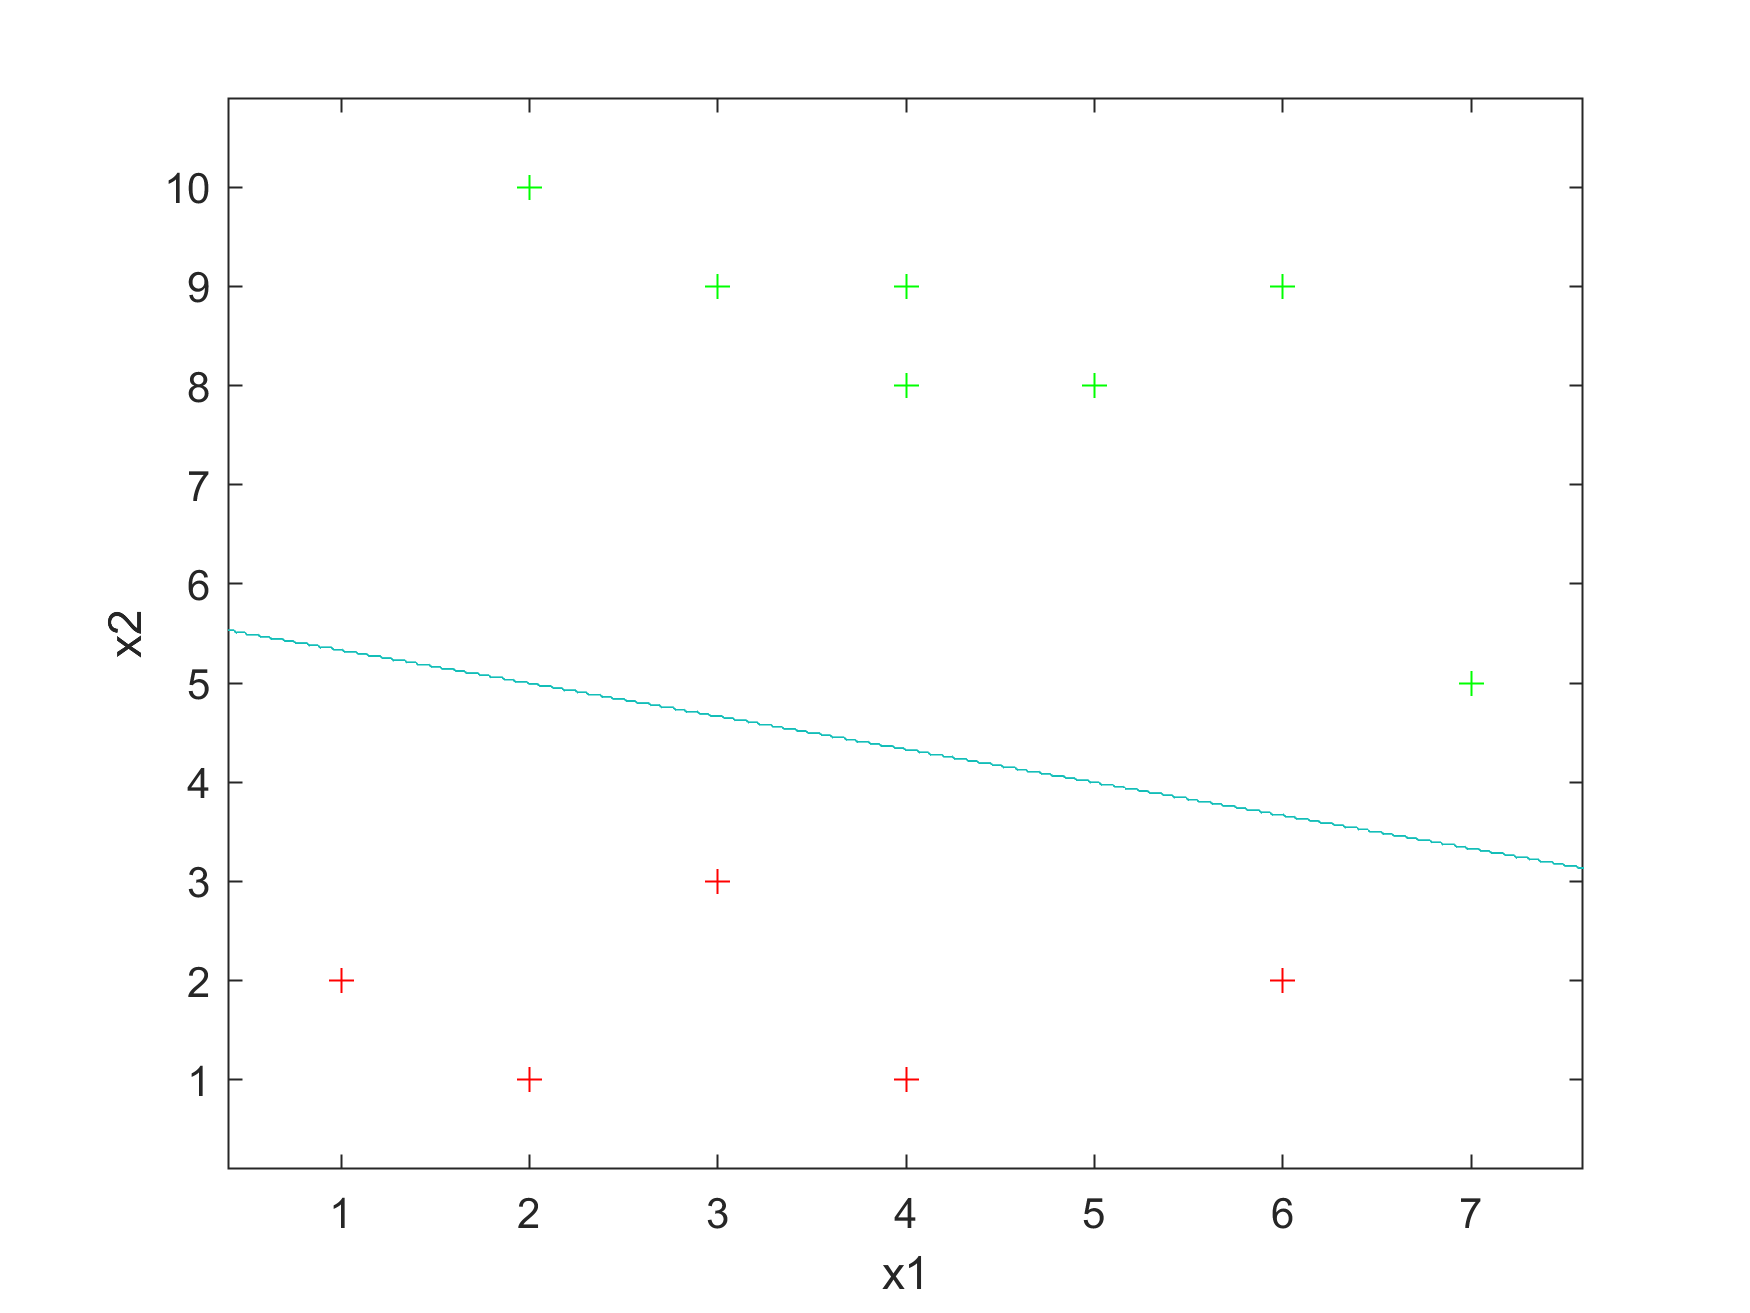
\includegraphics[width=\textwidth,height=0.7\textheight,keepaspectratio]{../code/octave/images/svmsimple}
            \caption{Beispiel Trenngrenze lineares Problem mit Hard-Margin SVM}
            \label{fig:bsphmsvm}
        \end{figure}
    \end{center}
\end{frame}

\begin{frame}{Vergleich Hard-Margin SVM}
    Vergleich mit $\alpha$-LMS, Algorithmus mit Pseudoinverse \\ \pause
    \begin{center}
        \begin{figure}
            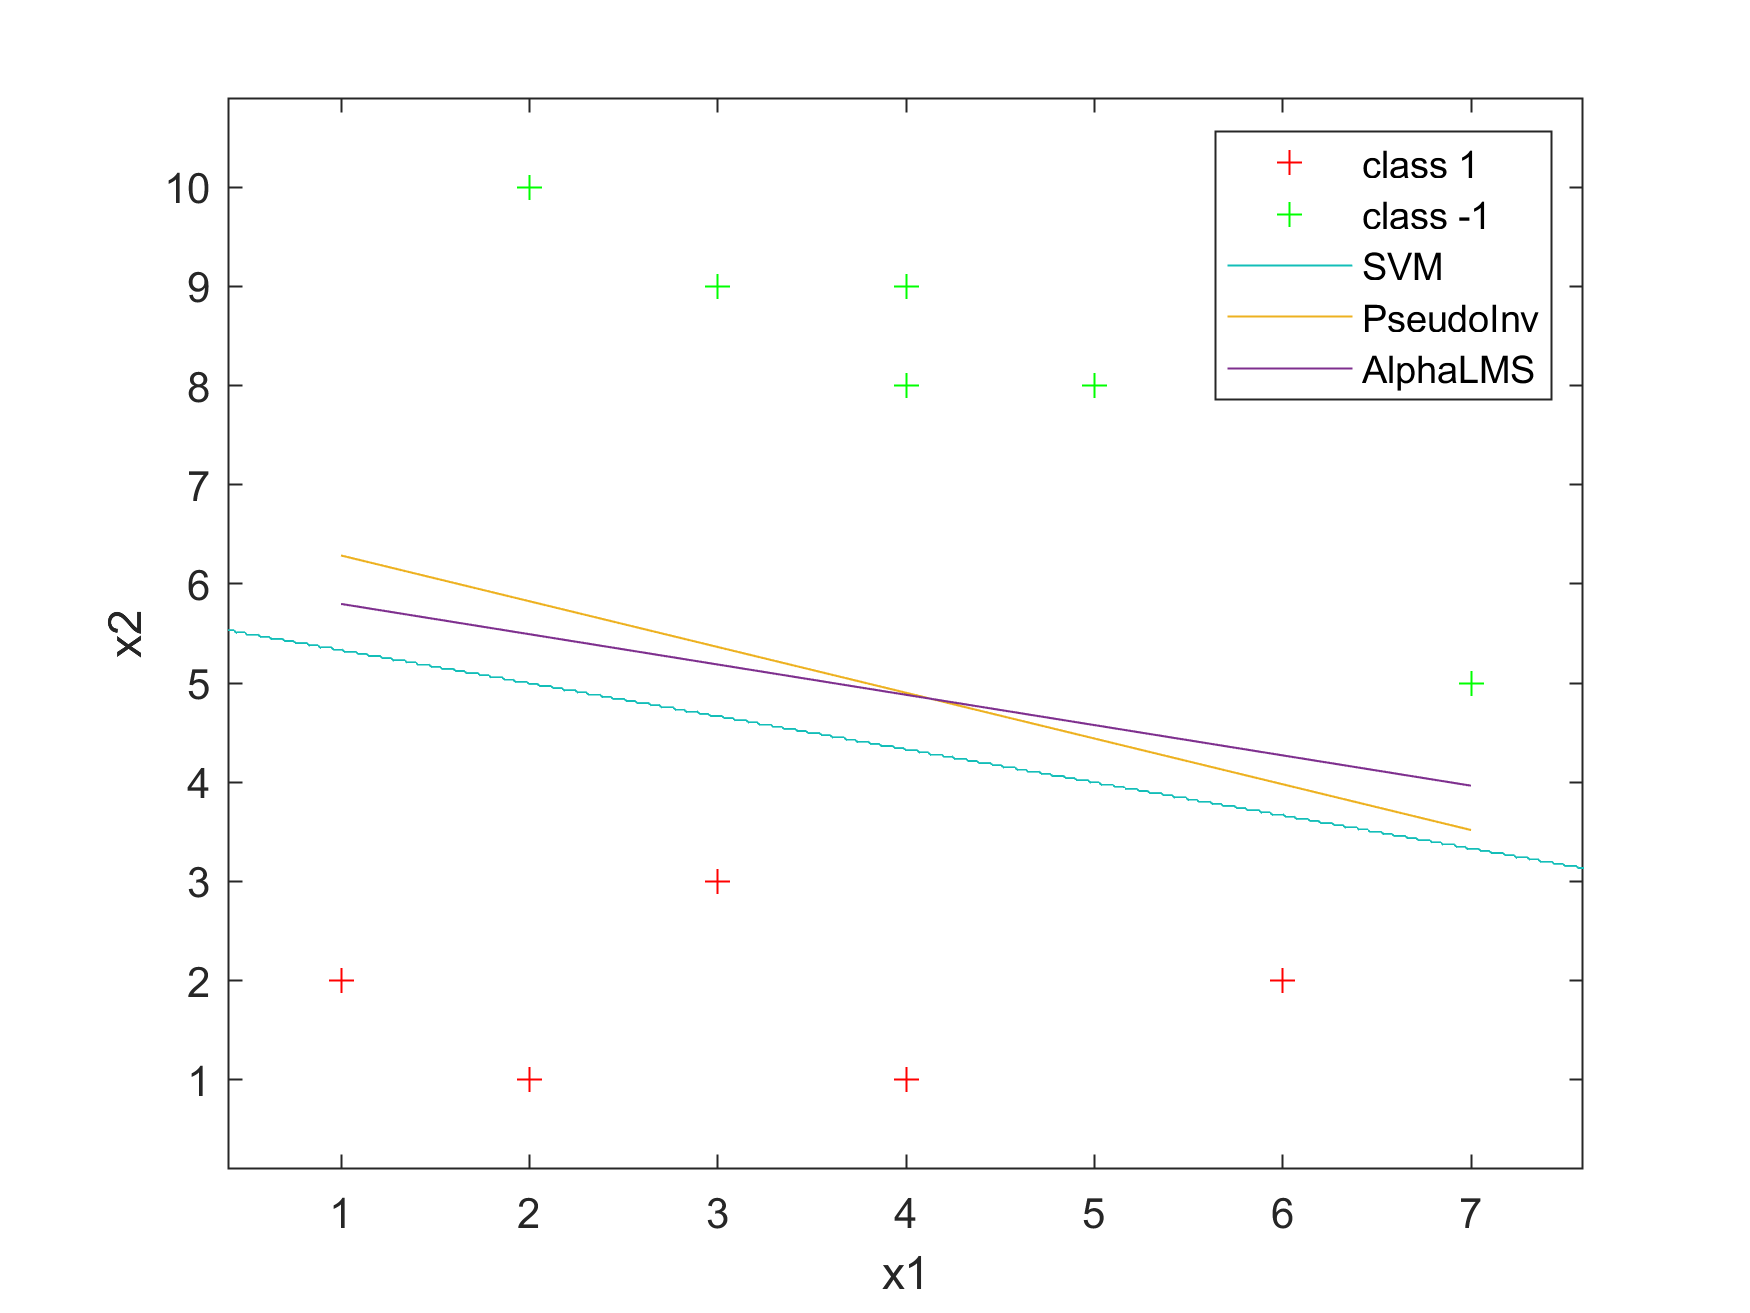
\includegraphics[width=\textwidth,height=0.7\textheight,keepaspectratio]{../code/octave/images/linearcompsmall}
            \caption{Vergleich Hard-Margin SVM, $\alpha$-LMS, Algo mit Pseudoinverse}
            \label{fig:comphardalphaps}
        \end{figure}
    \end{center}
\end{frame}

\begin{frame}{Pseudocode Soft-Margin SVM}
    \centering
    \begin{tabular}{l r}
        \textbf{Soft-Margin SVM} & \textbf{Zeile} \\
        \hline
        \textcolor{red}{Initialisiere $\mathbf{x}, \mathbf{y}, C$ }& 1\\ \pause
        $\mathbf{Q} = (\mathbf{y}\mathbf{y}^{\mathbf{T}})\mathbf{K}$ & 2\\
        $\mathbf{c} = \left( -1, -1, \ldots, -1 \right)^{\mathbf{T}}$ & 3 \\
        $\mathbf{A} = diag\left( -1, -1, \ldots, -1 \right)$ & 4 \\
        $\mathbf{b} = \left( 0, 0, \ldots, 0 \right)^{\mathbf{T}}$ & 5\\
        $\mathbf{A_{eq}} = \mathbf{y}^{\mathbf{T}}$ & 6\\
        $b_{eq} = 0$ & 7\\ \pause
        \textcolor{red}{$\mathbf{lb} = \left( 0, 0, \ldots, 0 \right)^{\mathbf{T}}$} & 8 \\
        \textcolor{red}{$\mathbf{ub} = C * \left( 1, 1, \ldots, 1 \right)^{\mathbf{T}}$} & 9 \\ \pause
        \textcolor{red}{$\mathbf{\alpha} = QPSolver\left( \mathbf{Q}, \mathbf{c}, \mathbf{A}, b, \mathbf{A_{eq}}, \mathbf{b_{eq}}, \mathbf{lb}, \mathbf{ub} \right)$} & 10\\ \pause
        $\mathbf{w} = \sum\limits_{n=SV} \alpha_{n} y_{n} x_{n}$  & 11\\
        & \\[-1em]
        $bias = \frac{1}{y_{n}} - \mathbf{w}^{\mathbf{T}}x_{n}$ & 12\\
    \end{tabular}
\end{frame}

\begin{frame}{QP Parameter Soft Margin}
    \centering
    $\!\min_{\alpha} \qquad \Lagr(\alpha) = \frac{1}{2} \alpha^{T} Q \alpha + (-1^T) \alpha$ \\ \pause
    $A \alpha \leq b$ -> $diag(-1) * \alpha \leq 0$ \\ \pause
    $A_{e q} \alpha = b_{e q}$ -> $y^{T} \alpha = 0$ \\ \pause
    $lb \leq \alpha \leq ub$ -> $0 \leq \alpha \leq C$
\end{frame}

\begin{frame}{Anmerkungen zu Pseudocode Soft-Margin SVM}
    \textbf{Anmerkungen} \\
    \begin{itemize}
        \item Zeile 1: Initialisieren von Werte- und Klassenvektoren und Bestrafungsparameter C
        \item Zeile 2: Berechnen der Matrix Q
        \item Zeile 3: Berechnen von c
        \item Zeile 4, 5: Berechnen der Ungleichheitsbedingungen
        \item Zeile 6, 7: Berechnen der Gleichheitsbedingungen
        \item Zeile 8: untere Grenze (kann auch $\left( -\infty, -\infty, \ldots, -\infty \right)$ gewählt werden)
        \item Zeile 9: Berechnung obere Grenze mit C
        \item Zeile 10: Lösen mittels Quadratic Programming
        \item Zeile 11: Berechnung Gewichte mit Stützvektoren
        \item Zeile 12: Berechnung bias mit beliebigem Stützvektor
    \end{itemize}
\end{frame}

\begin{frame}{Beispiel Soft-Margin SVM}
    \begin{columns}
        \begin{column}{0.8\textwidth}
        \begin{figure}
            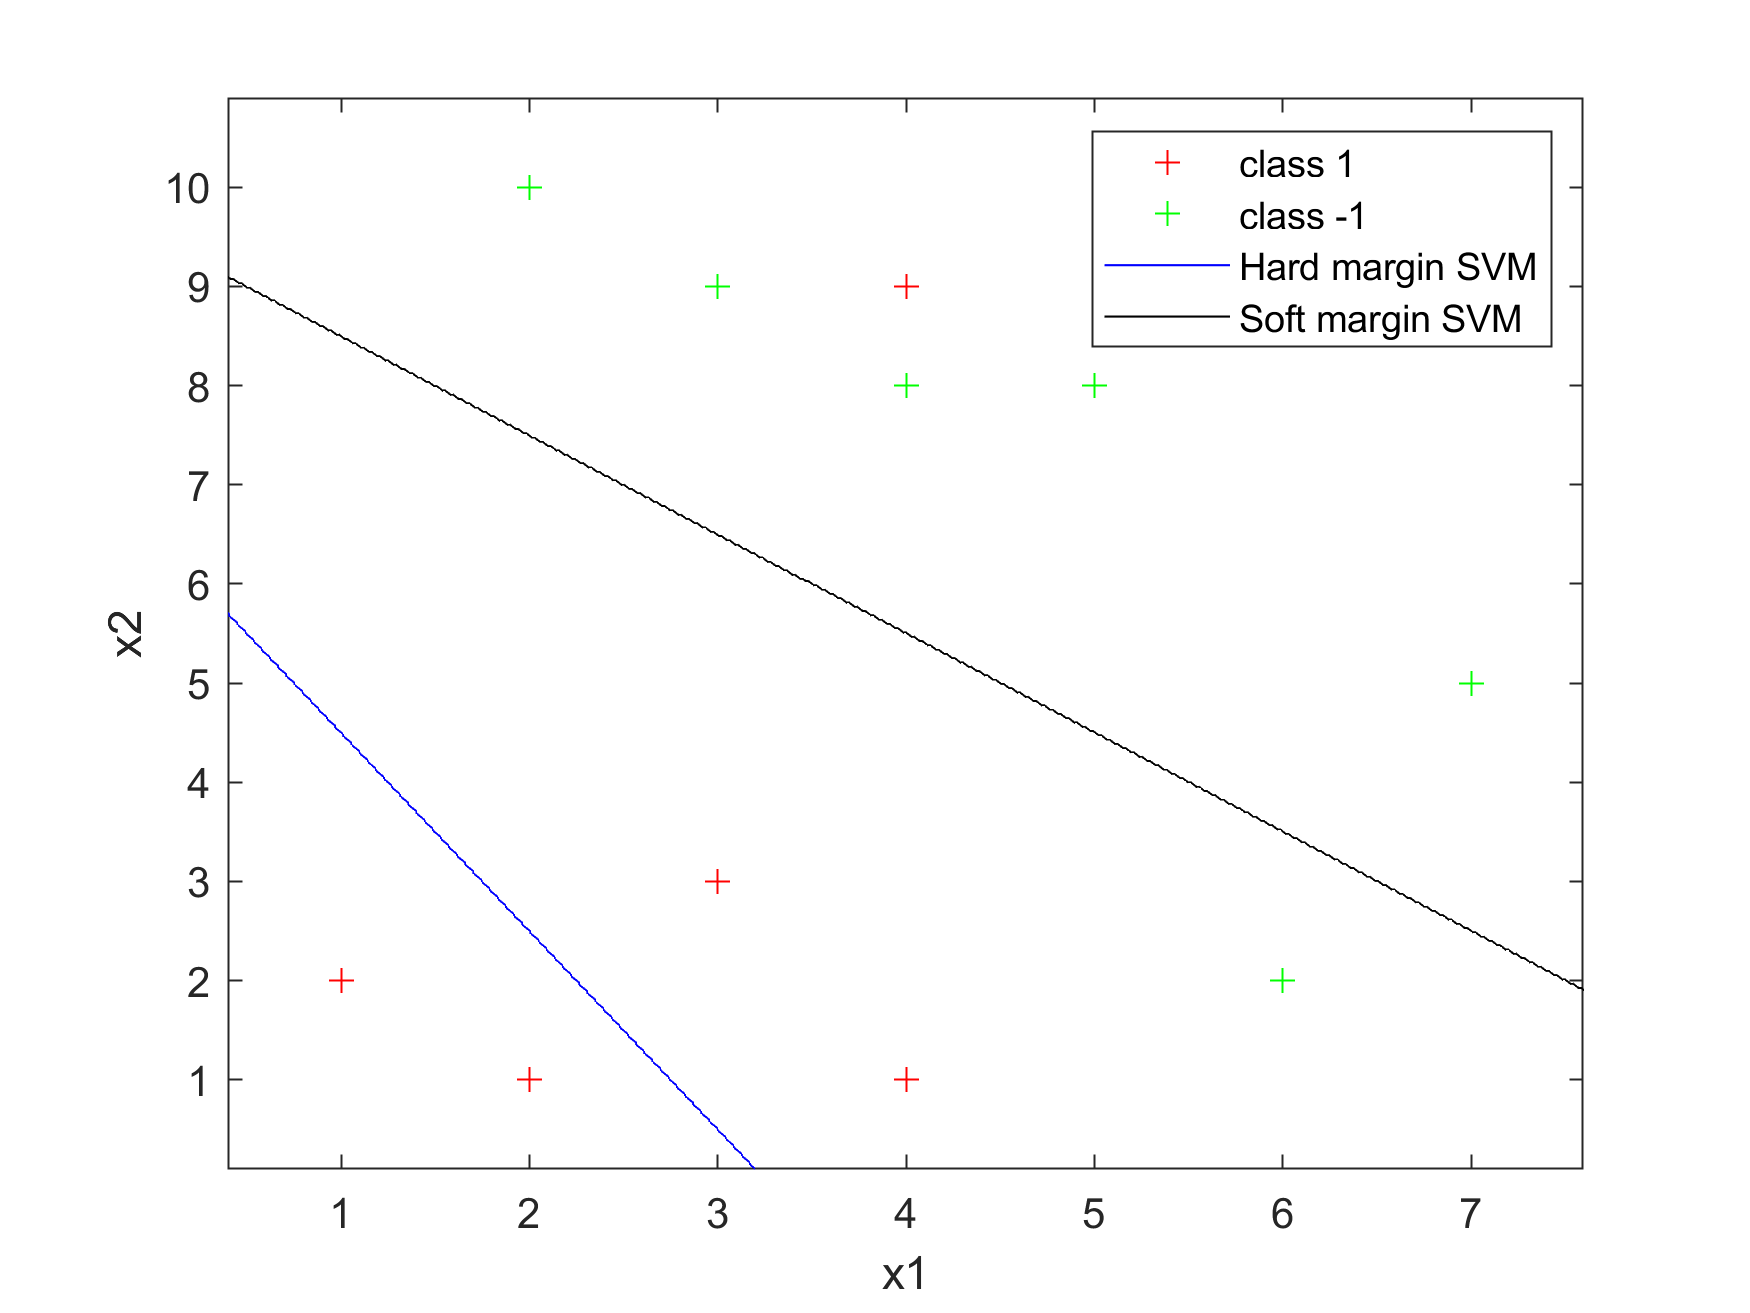
\includegraphics[width=\textwidth,height=\textheight,keepaspectratio]{../code/octave/images/svmsimplenotlinear}
            \caption{Trenngrenze nichtlineares Problem mit Hard-Margin und Soft-Margin SVM}
            \label{fig:bspsmsvm}
        \end{figure} \pause
        \end{column}
        \begin{column}{0.2\textwidth}
        Gute Ergebnisse auch bei Ausreißern
            \end{column}
    \end{columns}

\end{frame}

\begin{frame}{Pseudocode Kernel-Trick}
    \centering
    \begin{tabular}{l r}
        \textbf{Soft-Margin SVM mit Kernel-Trick} & \textbf{Zeile} \\
        \hline
        Initialisiere $\mathbf{x}, \mathbf{y}, C$ & 1\\ \pause
        \textcolor{red}{$\mathbf{Q} = (\mathbf{y}\mathbf{y}^{\mathbf{T}})\mathbf{K}$} & 2\\ \pause
        $\mathbf{c} = \left( -1, -1, \ldots, -1 \right)^{\mathbf{T}}$ & 3 \\
        $\mathbf{A} = diag\left( -1, -1, \ldots, -1 \right)$ & 4 \\
        $\mathbf{b} = \left( 0, 0, \ldots, 0 \right)^{\mathbf{T}}$ & 5\\
        $\mathbf{A_{eq}} = \mathbf{y}^{\mathbf{T}}$ & 6\\
        $b_{eq} = 0$ & 7\\
        $\mathbf{lb} = \left( 0, 0, \ldots, 0 \right)^{\mathbf{T}}$ & 8 \\
        $\mathbf{ub} = C * \left( 1, 1, \ldots, 1 \right)^{\mathbf{T}}$ & 9 \\
        $\mathbf{\alpha} = QPSolver\left( \mathbf{Q}, \mathbf{c}, \mathbf{A}, b, \mathbf{A_{eq}}, \mathbf{b_{eq}}, \mathbf{lb}, \mathbf{ub} \right)$ & 10\\ \pause
        \textcolor{red}{$bias = y_{k} - \sum\limits_{\alpha_{n} > 0} \alpha_{n} y_{n} KF\left( x_{n}, x_{k} \right) $} & 11 \\
    \end{tabular}
\end{frame}

\begin{frame}{Anmerkungen zu Pseudocode Kernel-Trick}
    \textbf{Anmerkungen} \\
    \begin{itemize}
        \item $KF$ ist die Kernel-Funktion.
        \item Algorithmus ist für alle Kernel (RBF, polynomiell, \ldots) gleich.
        \item Klassifizierung muss auch angepasst werden.
        \item Zeile 1: Initialisieren von Werte- und Klassenvektoren und Bestrafungsparameter C
        \item Zeile 2: Berechnen der Matrix Q
        \item Zeile 3: Berechnen von c
        \item Zeile 4, 5: Berechnen der Ungleichheitsbedingungen
        \item Zeile 6, 7: Berechnen der Gleichheitsbedingungen
        \item Zeile 8: untere Grenze (kann auch $\left( -\infty, -\infty, \ldots, -\infty \right)$ gewählt werden)
        \item Zeile 9: Berechnung obere Grenze mit C
        \item Zeile 10: Lösen mittels Quadratic Programming
        \item Zeile 11: Berechnung bias, $x_{k}$ ist ein beliebiger Stützvektor, $y_{k}$ die dazugehörende Klasse. Aufgrund von Rechenungenauigkeiten empfiehlt sich ein Vergleich von $\alpha_{n}$ mit nicht exakt $0$, sondern einem sehr kleinen Wert, e.g. $10^{-10}$
    \end{itemize}
\end{frame}

\begin{frame}{Pseudocode für $K$-Matrix bei Kernel}
    \centering
    \begin{tabular}{l r}
        $\mathbf{K}$ \textbf{Berechnung} & \textbf{Zeile} \\
        \hline
        Initialisiere $\mathbf{x}$ & 1 \\
        For $i=1$ To $N$ & 2 \\
        \quad For $j=1$ To $N$ & 3 \\ \pause
        \textcolor{red}{\quad\quad $\mathbf{K}\left( i, j \right) = KF\left( x_{i}, x_{j} \right)$} & 4 \\
        \quad Ende For & 5 \\
        Ende For & 6 \\
    \end{tabular} \pause \\
    \vspace{\baselineskip}
    $N$ Anzahl Eingabevektoren, $KF$ Kernel-Funktion \\
    Anstatt Skalarprodukt Kernel-Funktion \\
    Spart Transformation in höhere Dimensionen
\end{frame}

\begin{frame}{Beispiel Polynomieller Kernel}
    Kernel: $(a x^{T}x' + b)^{Q}$, $b = 1, a = 1$, Exponent $Q$ wird variiert \\ \pause
        \begin{figure}
            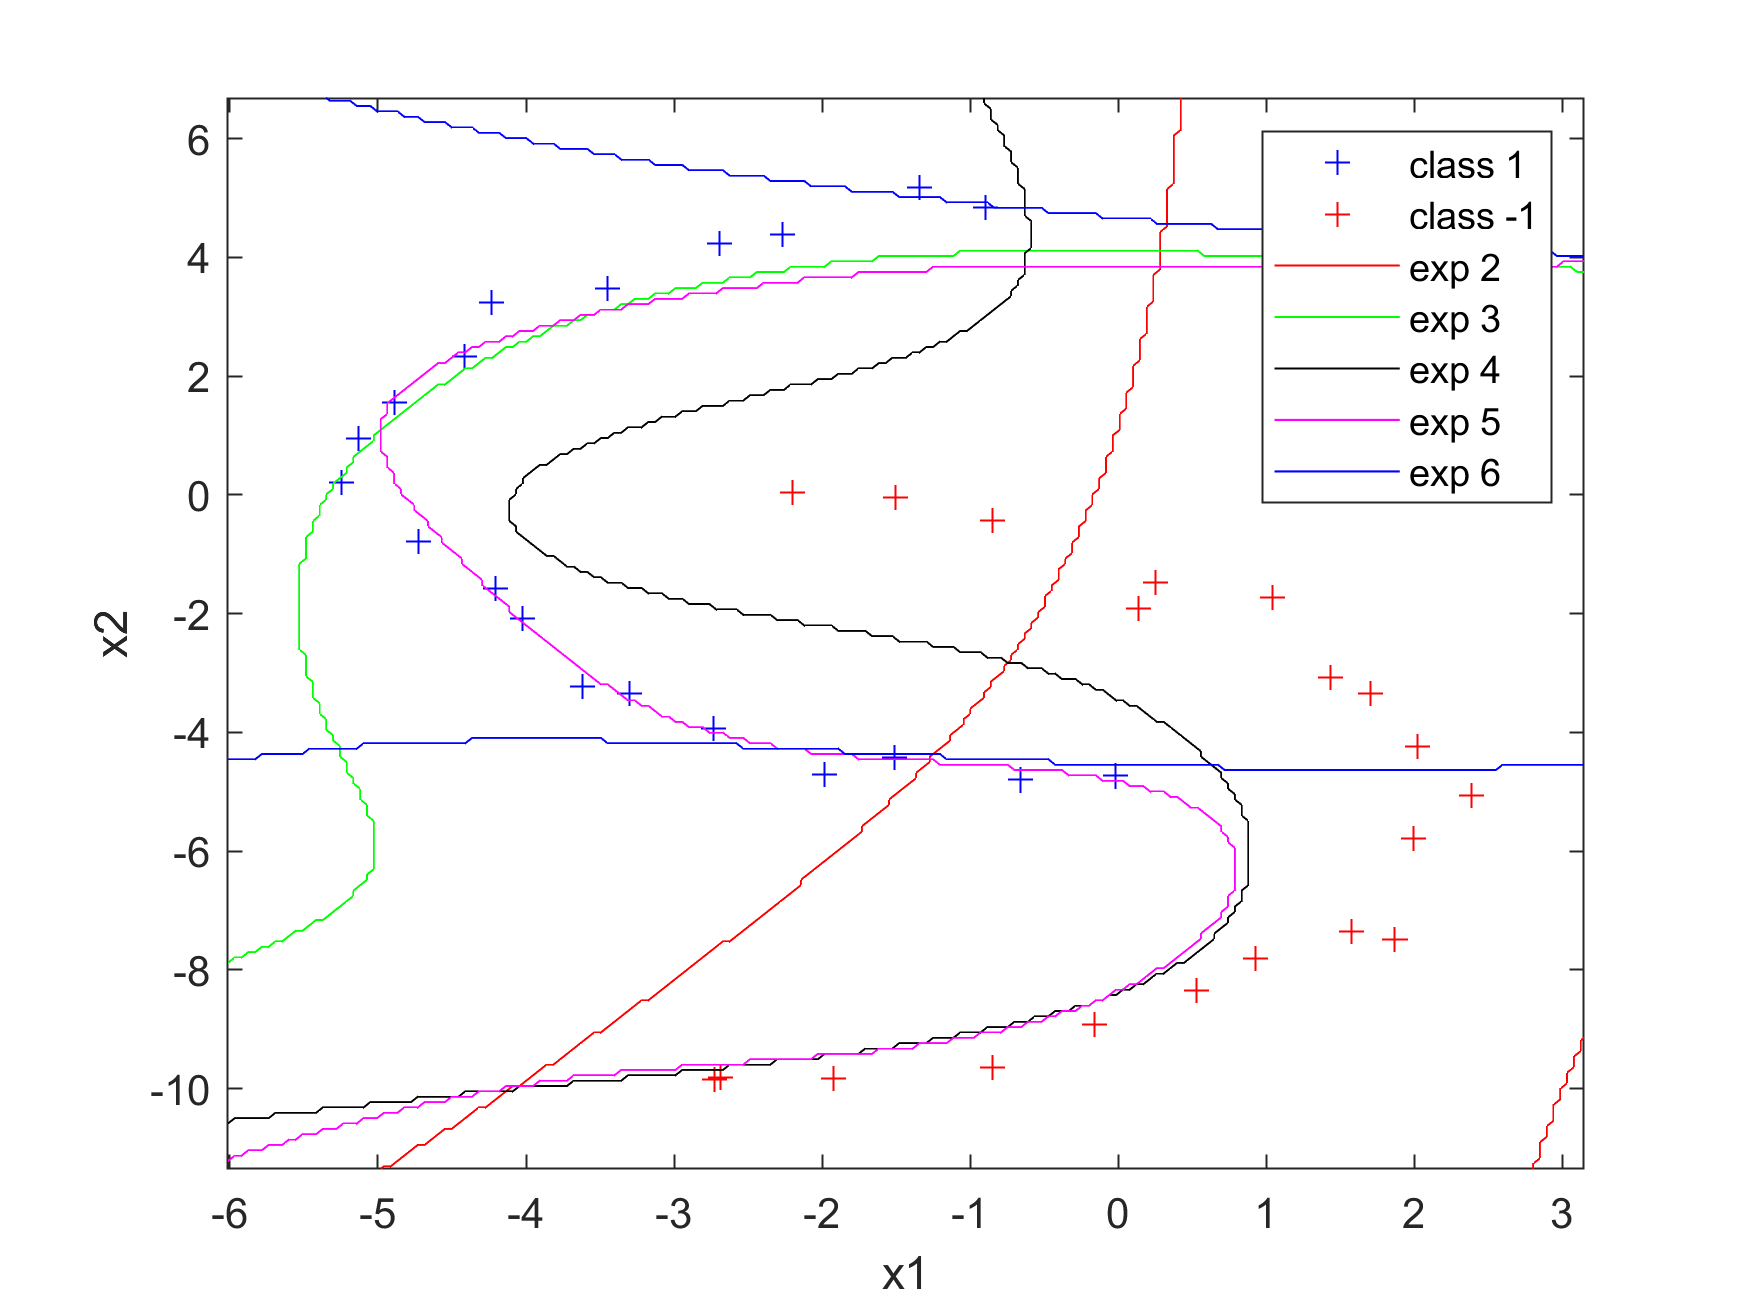
\includegraphics[width=\textwidth,height=0.7\textheight,keepaspectratio]{../code/octave/images/kernelexptest}
            \caption{Trenngrenzen für polynomiellen Kernel mit verschiedenen Exponenten $Q$}
            \label{fig:bsppolykern}
        \end{figure}
\end{frame}

\begin{frame}{Beispiel Polynomieller Kernel mit $Q=4$}
    \begin{center}
        \begin{figure}
            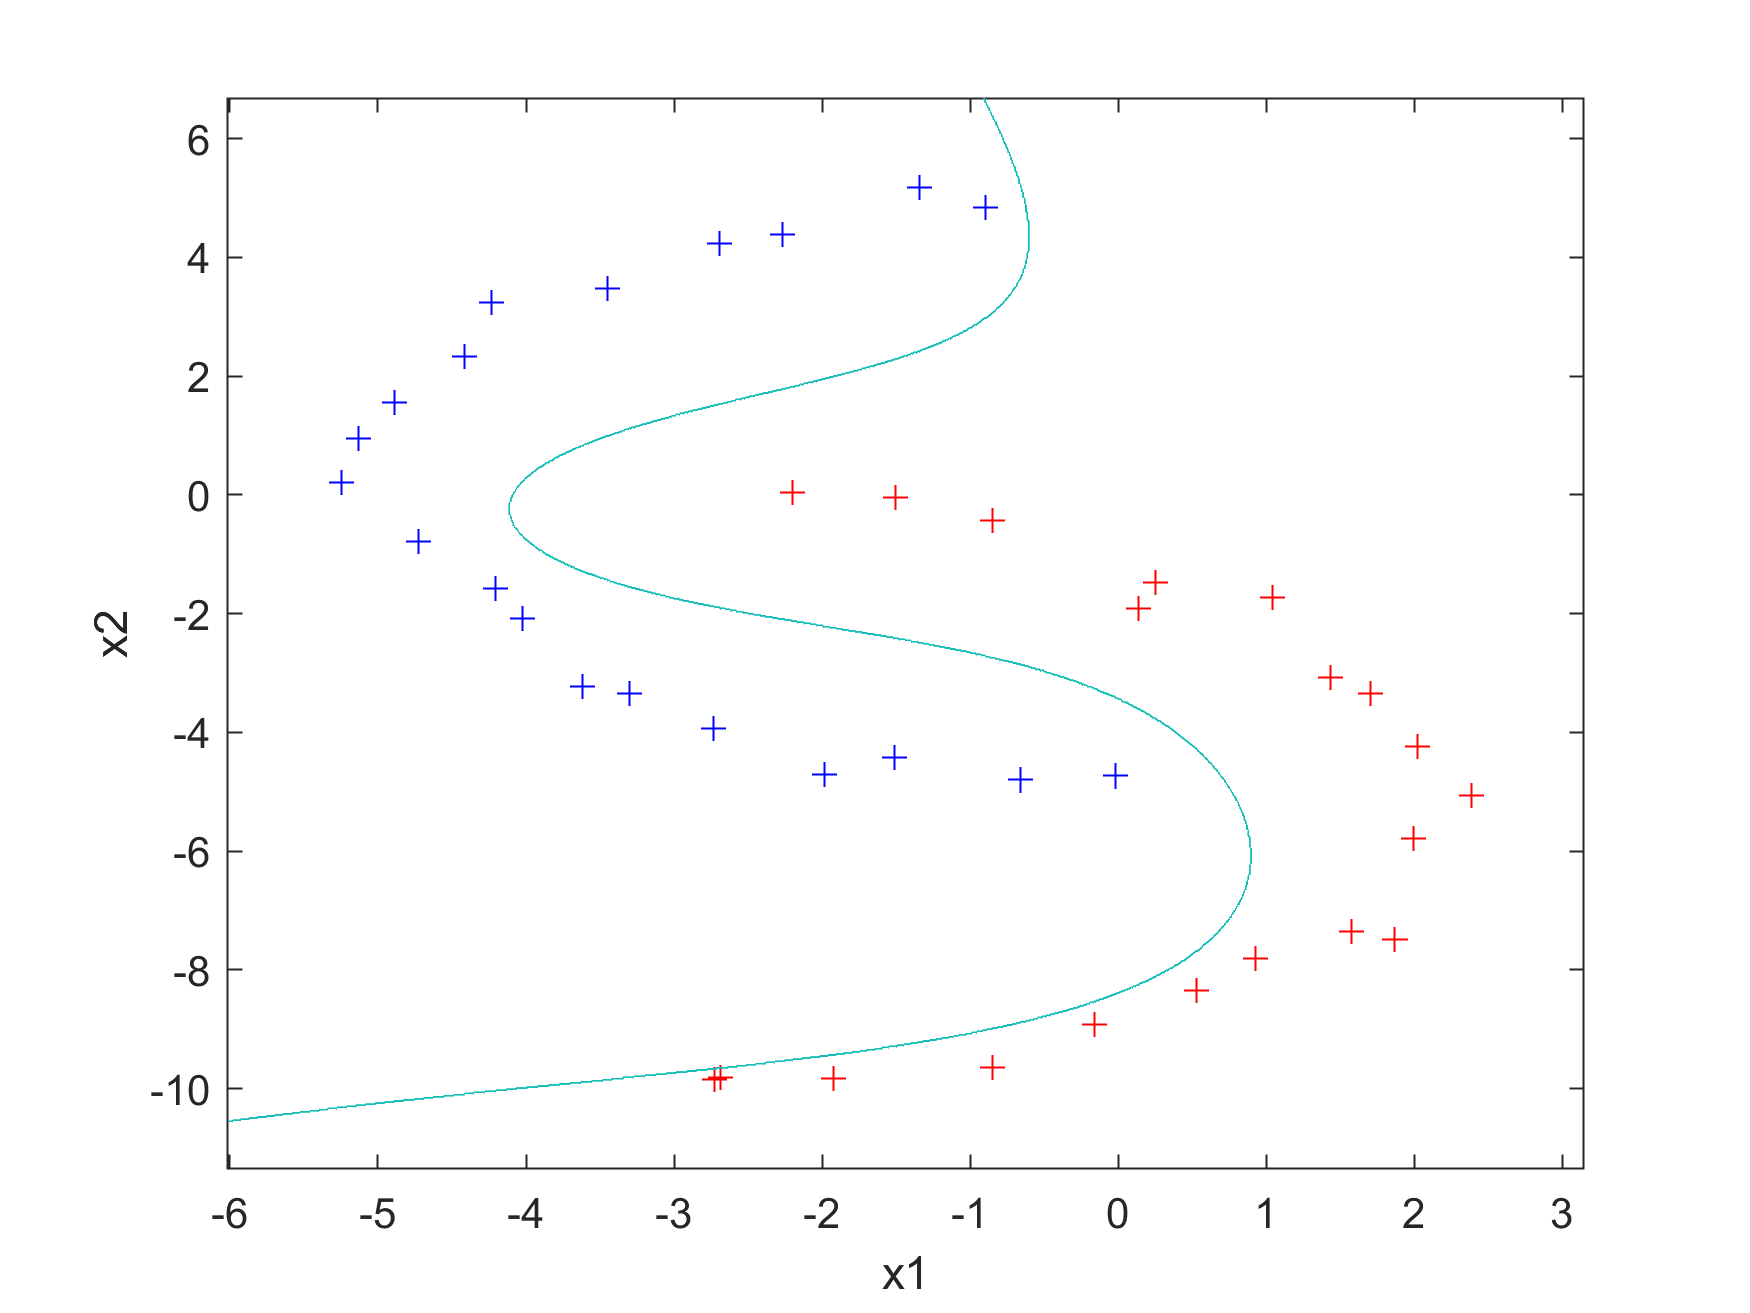
\includegraphics[width=\textwidth,height=0.7\textheight,keepaspectratio]{../code/octave/images/sgddatasetkernelsolve}
            \caption{Trenngrenzen für polynomiellen Kernel $(a x^{T}x' + b)^{Q}$ mit $Q=4$}
            \label{fig:bsppolykernqfour}
        \end{figure}
    \end{center}
\end{frame}

\begin{frame}{Beispiel RBF Kernel, verschiedene $\gamma$}
    Parameter $\gamma$ muss richtig eingestellt werden \pause
    \begin{columns}
        \begin{column}{0.8\textwidth}
            \begin{figure}
                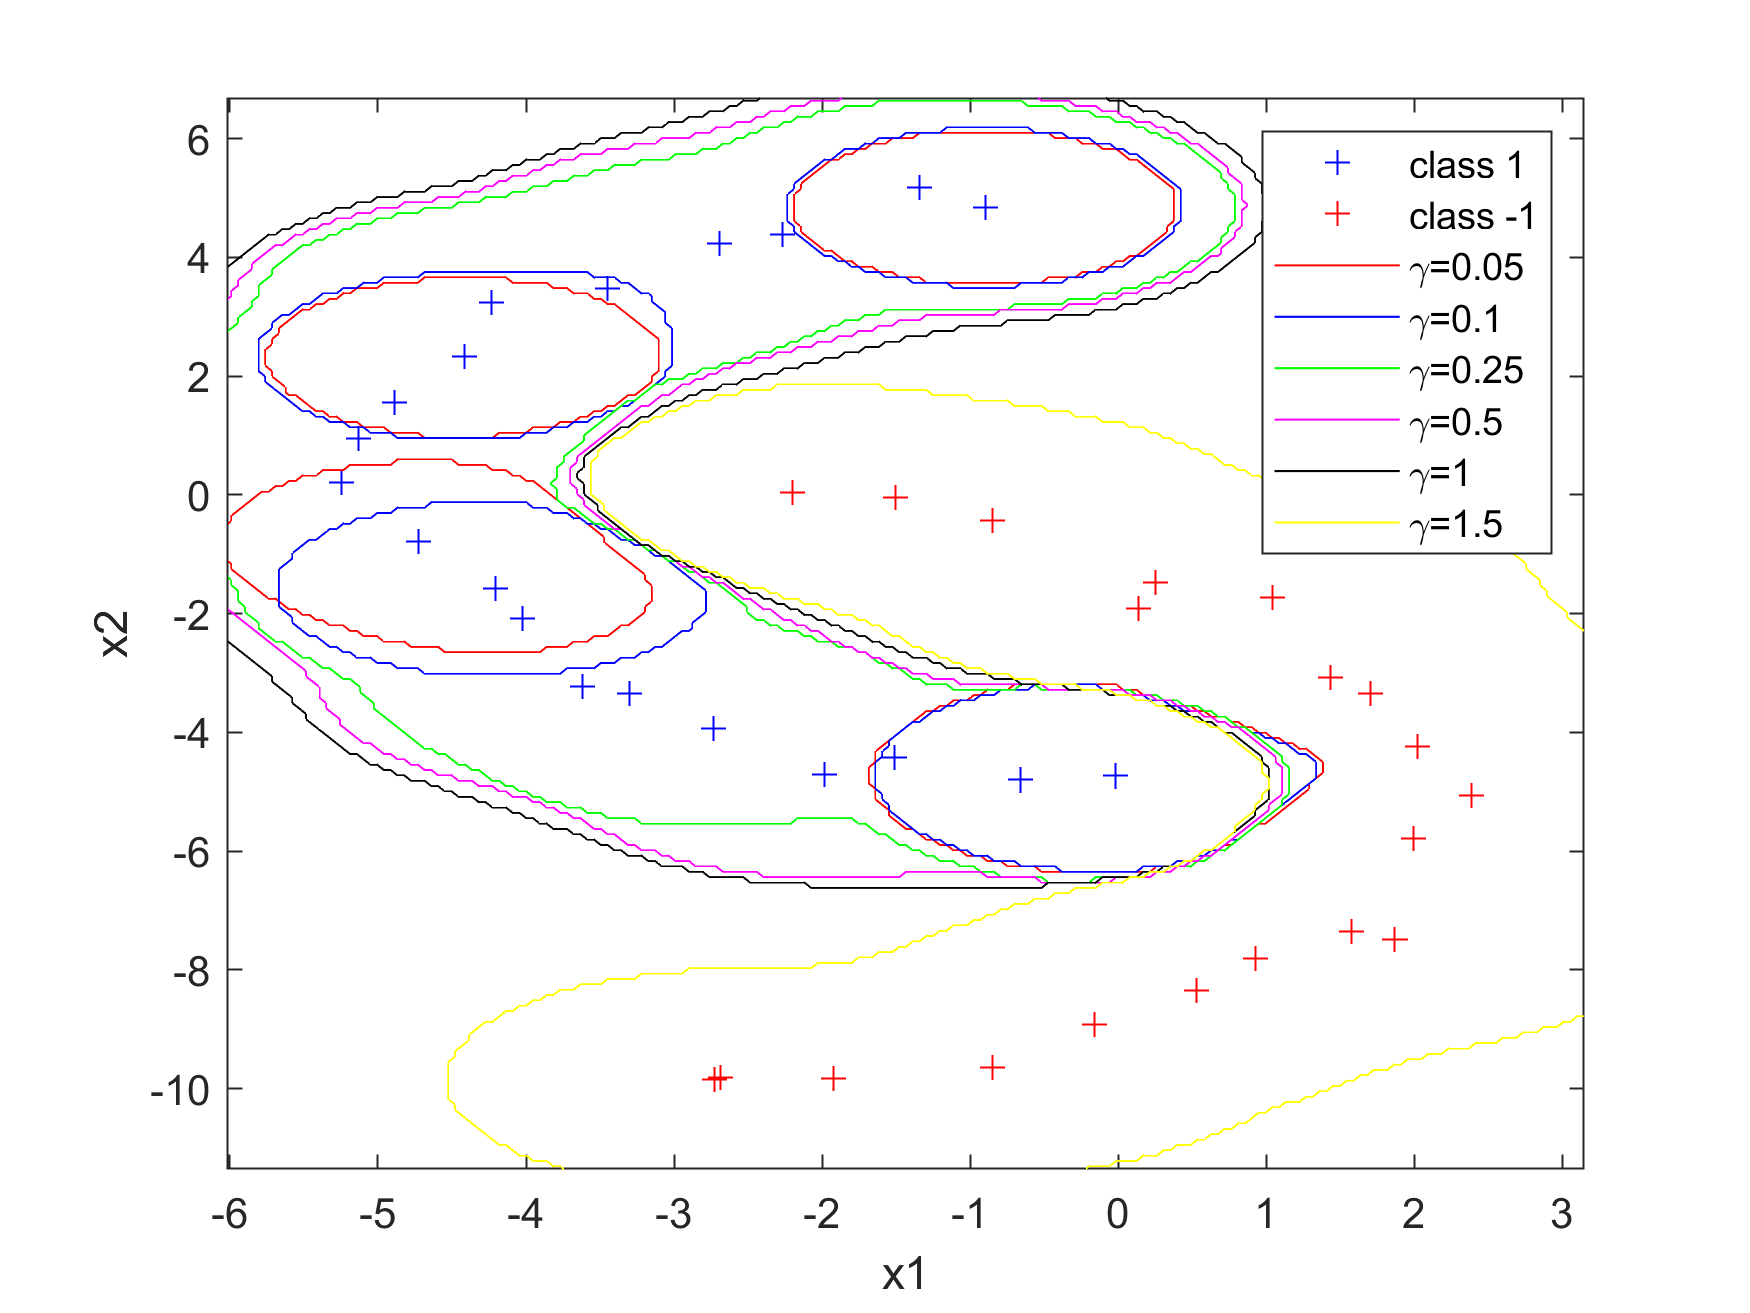
\includegraphics[width=\textwidth,height=0.7\textheight,keepaspectratio]{../code/octave/images/sgdrbfkernelcomp}
                \caption{Trenngrenzen für RBF Kernel mit verschiedenen $\gamma$}
                \label{fig:bsprbfkernelcomp}
            \end{figure}
        \end{column} \pause
        \begin{column}{0.2\textwidth}
            Bei falschem $\gamma$ zu kleine Gebiete \\ \pause
            \vspace{\baselineskip}
            $\gamma$ gut -> eine Klasse umschlossen
        \end{column}
    \end{columns}
\end{frame}

\begin{frame}{Beispiel RBF Kernel, $\gamma=1$}
    Parameter $\gamma=1$ \\ \pause
    \begin{columns}
        \begin{column}{0.8\textwidth}
        \begin{figure}
            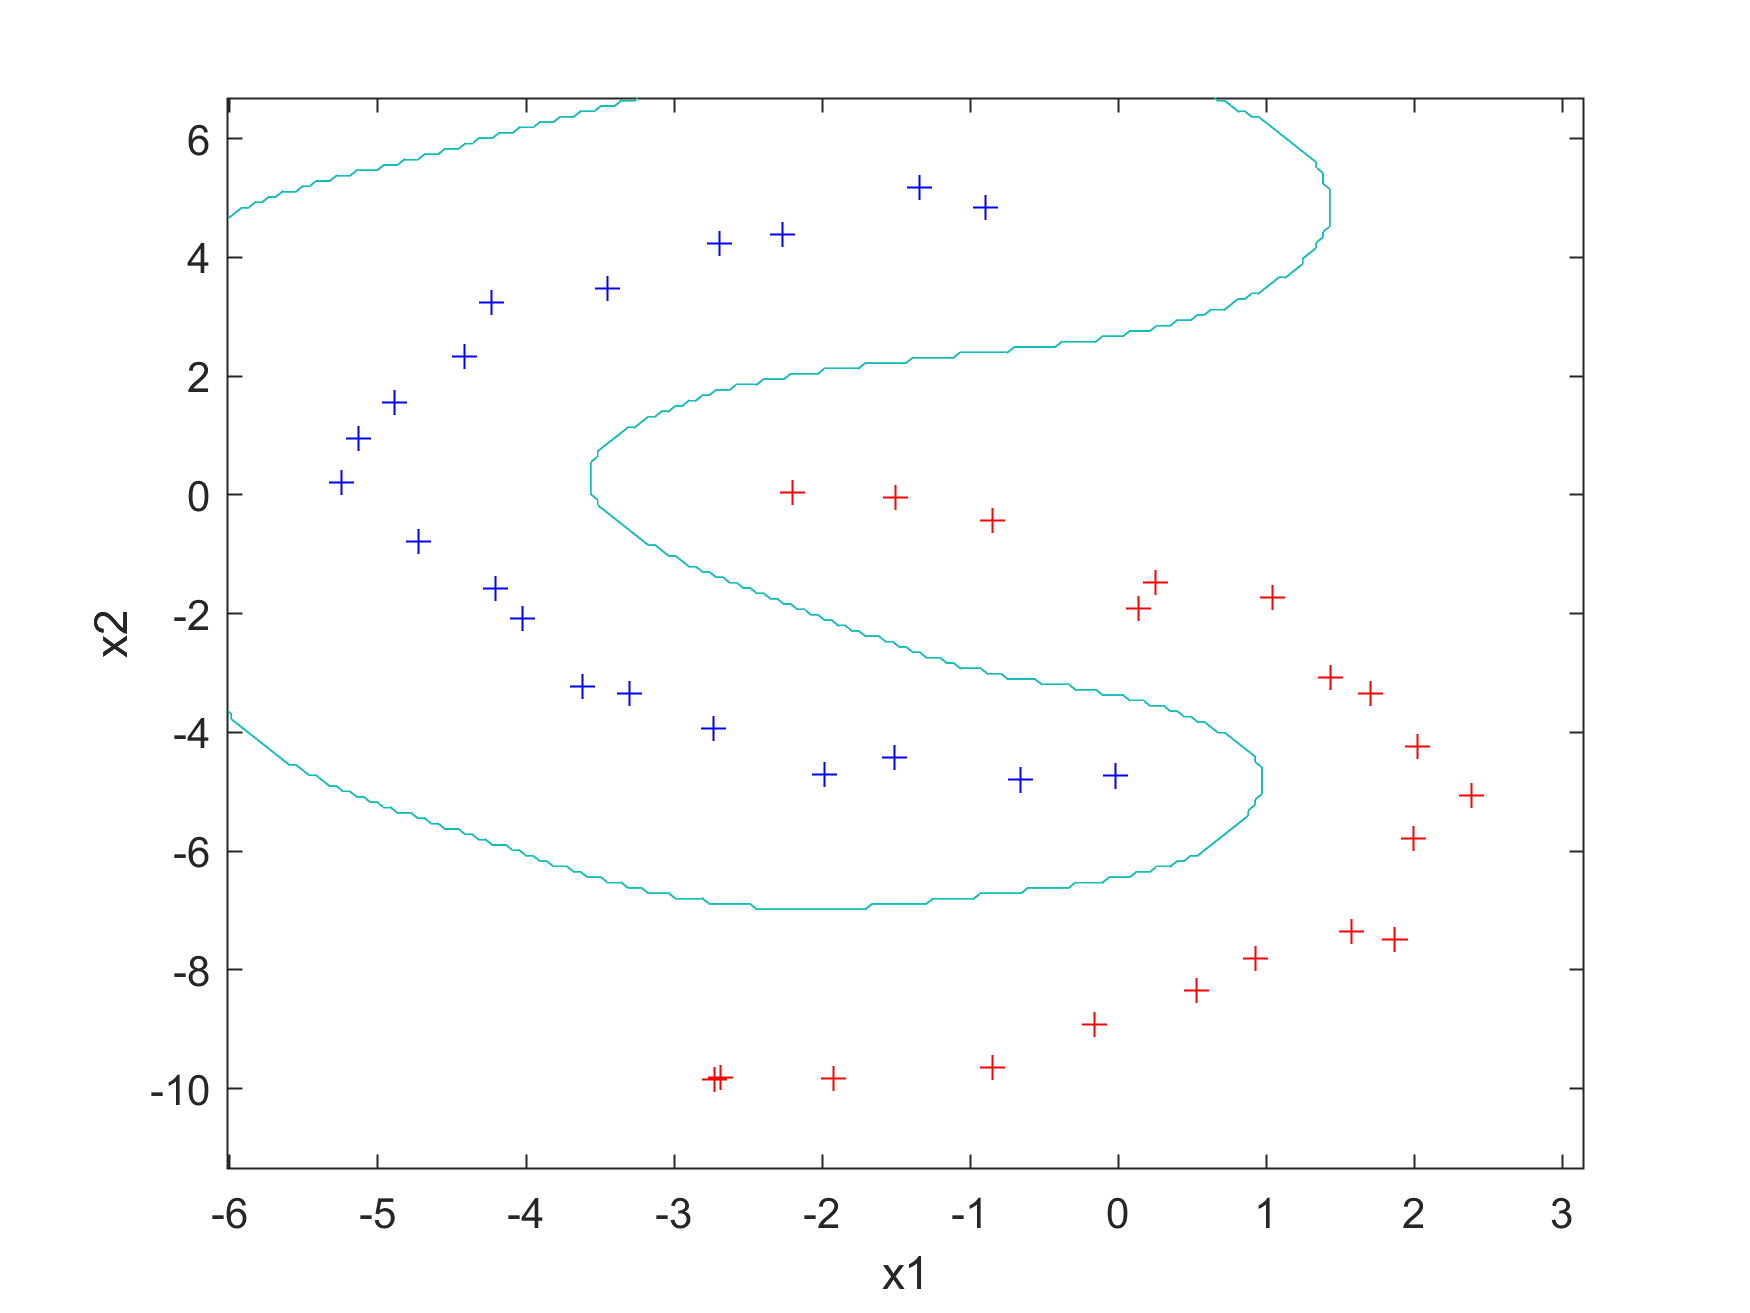
\includegraphics[width=\textwidth,height=0.7\textheight,keepaspectratio]{../code/octave/images/sgdrbfkernel}
            \caption{Trenngrenzen für RBF Kernel mit $\gamma=1$}
            \label{fig:bsprbfkernel}
        \end{figure}
    \end{column} \pause
        \begin{column}{0.2\textwidth}
    Blaue Punkte umschlossen
            \end{column}
        \end{columns}
\end{frame}

\begin{frame}{Vergleich verschiedener Algorithmen}
            \begin{figure}
                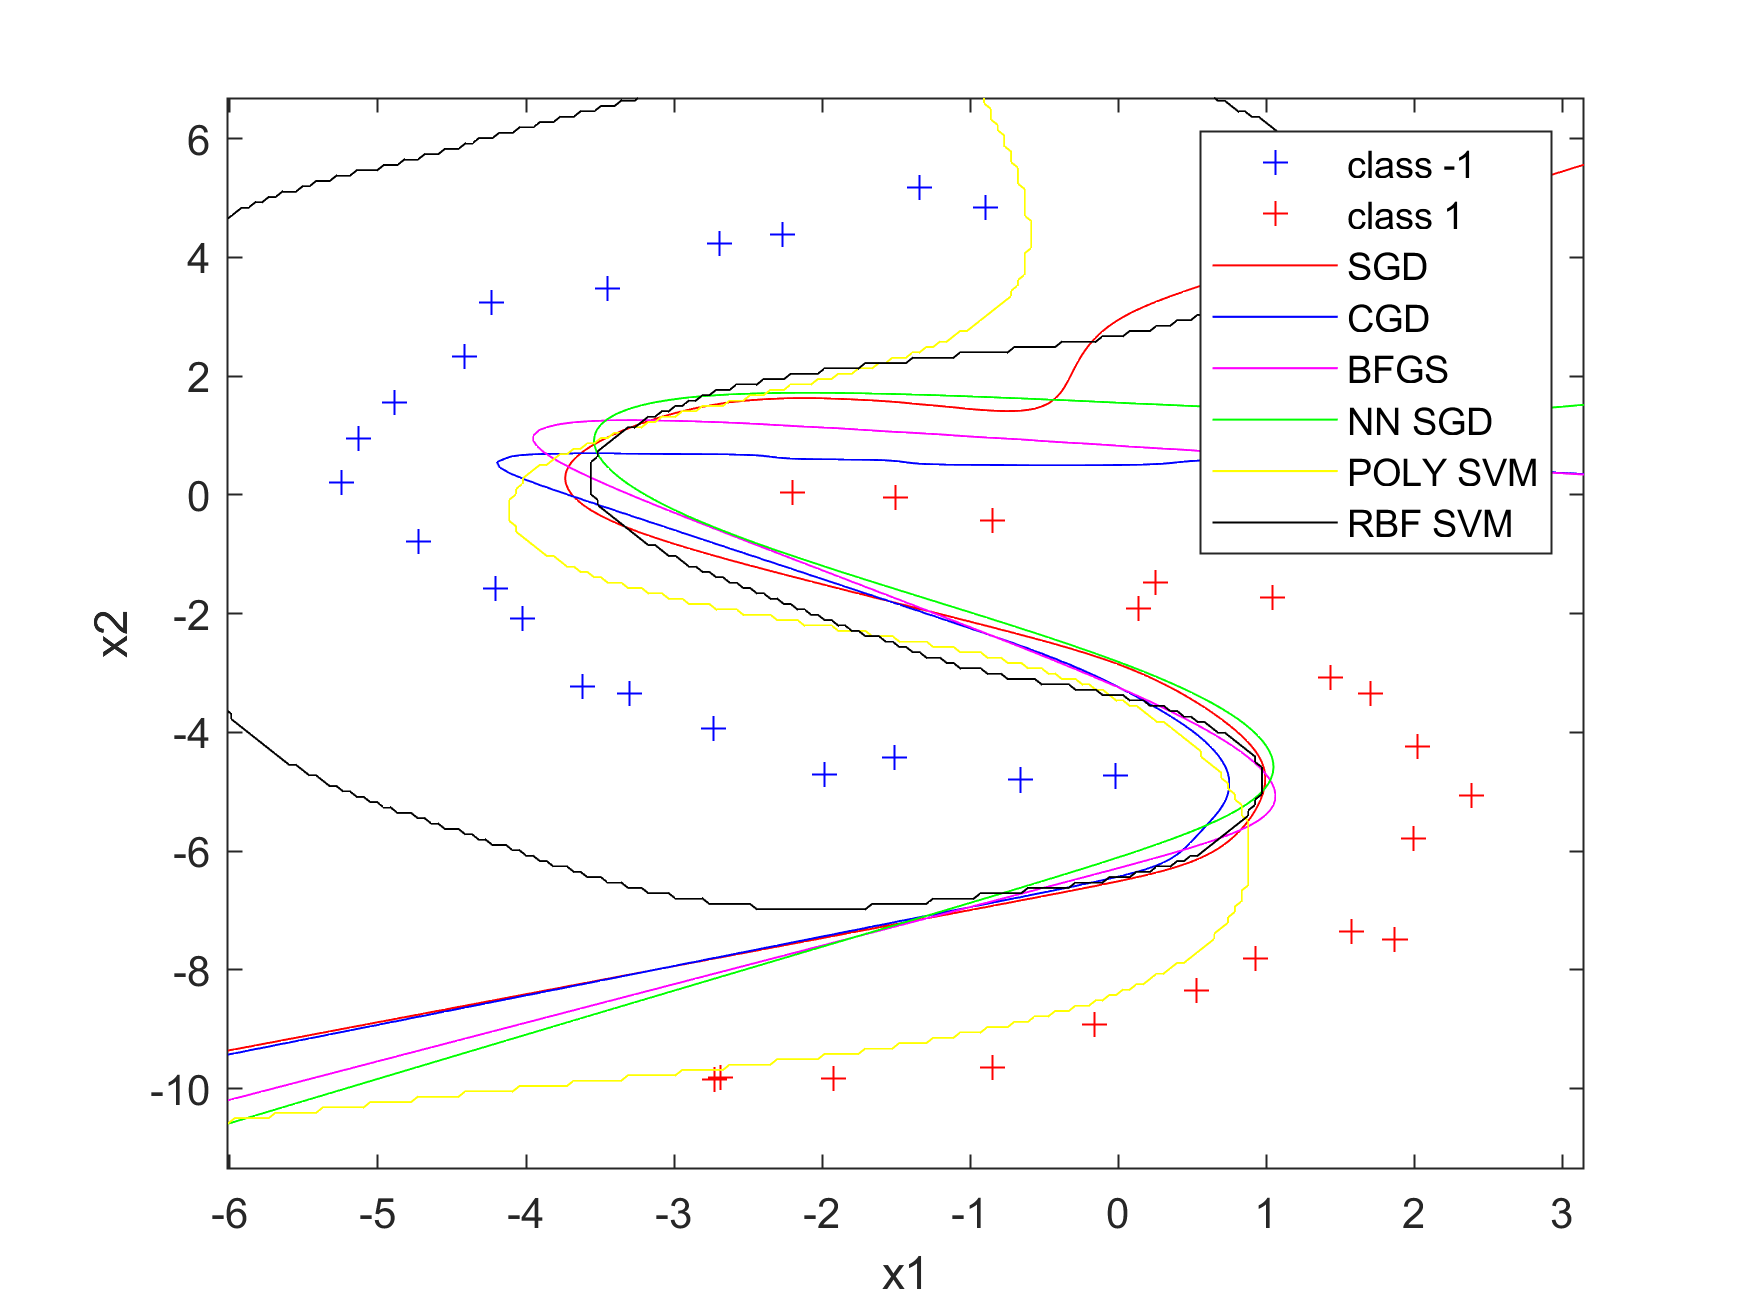
\includegraphics[width=\textwidth,height=0.7\textheight,keepaspectratio]{../code/octave/images/compbatchdecisionboundary}
                \caption{Trenngrenzen für verschiedene Methoden}
                \label{fig:vergleichalgos}
            \end{figure}
\end{frame}

\begin{frame}{Vergleich verschiedener Algorithmen}
    \begin{columns}
        \begin{column}{0.4\textwidth}
            \begin{figure}
                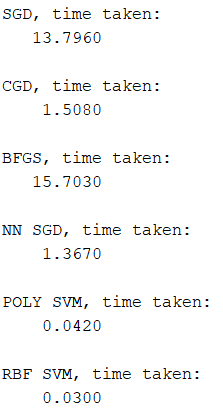
\includegraphics[width=\textwidth,height=0.7\textheight,keepaspectratio]{../code/octave/images/compbatchtimes}
                \caption{Dauer verschiedener Algorithmen}
                \label{fig:daueralgos}
            \end{figure}
        \end{column} \pause
        \begin{column}{0.6\textwidth}
            \begin{itemize}
                \item SVM sehr schnell \pause
                \item QP-Solver spielt entscheidende Rolle \pause
                \item SVM stabiler -> keine zufällig initialisierte Gewichtsmatrix \pause
                \item Experimente für Hyperparameter schnell und stabil
            \end{itemize}
        \end{column}
    \end{columns}
\end{frame}

\begin{frame}{Zusammenfassung}
    \centering
    \begin{itemize}
        \item SVM für lineare, binäre Klassifikationsprobleme \pause
        \item Hard und Soft Margin (Soft vermindert Einfluss Ausreißer) \pause
        \item Optimierungsproblem -> Lösen mit QP-Solver \pause
        \item Nichtlinear nur durch Transformation Eingabevektoren \pause
        \item Kernel Trick zum Umgehen der Transformation \pause
        \item Schnell, deterministisch
    \end{itemize}

\end{frame}

\begin{frame}[standout]
	Fragen?
\end{frame}

\end{document}



